%%%%%%%%%%%%%%%%%%%%%%%%%%%%%%%%%%%%%%%%%
% University Assignment Title Page 
% LaTeX Template
% Version 1.0 (27/12/12)
%
% This template has been downloaded from:
% http://www.LaTeXTemplates.com
%
% Original author:
% WikiBooks (http://en.wikibooks.org/wiki/LaTeX/Title_Creation)
%
% License:
% CC BY-NC-SA 3.0 (http://creativecommons.org/licenses/by-nc-sa/3.0/)
% 
% Instructions for using this template:
% This title page is capable of being compiled as is. This is not useful for 
% including it in another document. To do this, you have two options: 
%
% 1) Copy/paste everything between \begin{document} and \end{document} 
% starting at \begin{titlepage} and paste this into another LaTeX file where you 
% want your title page.
% OR
% 2) Remove everything outside the \begin{titlepage} and \end{titlepage} and 
% move this file to the same directory as the LaTeX file you wish to add it to. 
% Then add \input{./title_page_1.tex} to your LaTeX file where you want your
% title page.
%
%%%%%%%%%%%%%%%%%%%%%%%%%%%%%%%%%%%%%%%%%
%\title{Title page with logo}
%----------------------------------------------------------------------------------------
%	PACKAGES AND OTHER DOCUMENT CONFIGURATIONS
%----------------------------------------------------------------------------------------

\documentclass[11pt]{article}
\usepackage{amsmath}
\usepackage[left=2.5cm, right=2.5cm, top=3cm, bottom=3cm]{geometry}
\usepackage[utf8]{inputenc}
\usepackage[English]{babel}
\usepackage{amsmath}
\usepackage{fancyref}
\usepackage{graphicx}
\usepackage{float}
\usepackage{epigraph}
\usepackage{ragged2e}

%Paquetes necesarios para imágenes, pies de página, etc.
\usepackage{lmodern}
\usepackage{fancyhdr}



\usepackage{titlesec}

\titleformat{\section}
{\normalfont\Large\bfseries}{\thesection}{1em}{}
\titleformat{\subsection}
{\normalfont\large\bfseries}{\thesubsection}{1em}{}


%Modificación del formato de los captions
\usepackage[margin=10pt,labelfont=bf]{caption}
%Paquete para incluir hipervínculos
\usepackage[colorlinks=true, 
            linkcolor = blue,
            urlcolor  = blue,
            citecolor = black,
            anchorcolor = blue]{hyperref}

\usepackage[colorinlistoftodos]{todonotes}
\renewcommand{\baselinestretch}{1.2} 
\begin{document}

\begin{titlepage}

\newcommand{\HRule}{\rule{\linewidth}{0.5mm}} % Defines a new command for the horizontal lines, change thickness here

\center % Center everything on the page
 
%----------------------------------------------------------------------------------------
%	HEADING SECTIONS
%----------------------------------------------------------------------------------------

\begin{figure}[!h]
    \centering
    
\includegraphics[width=80pt]{logo.png}
    \label{fig:my_label}
\end{figure}


\textsc{\LARGE Universidad de los Andes}\\[2 cm] % Name of your university/college
% \textsc{\Large Presentación del 30 \%}\\[0.5cm] % Major heading such as course name
% \textsc{\large Minor Heading}\\[0.5cm] % Minor heading such as course title

%----------------------------------------------------------------------------------------
%	TITLE SECTION
%----------------------------------------------------------------------------------------

\HRule \\[0.4cm]
{ \huge \bfseries Supercluster characterization in cosmological simulations}\\[0.4cm] % Title of your document
\HRule \\[1.5cm]
 
%----------------------------------------------------------------------------------------
%	AUTHOR SECTION
%----------------------------------------------------------------------------------------

\begin{minipage}{0.4\textwidth}
\begin{flushleft} \large
\emph{Author:}\\
David L. \textsc{Paipa} % Your name
\end{flushleft}
\end{minipage}
~
\begin{minipage}{0.4\textwidth}
\begin{flushright} \large
\emph{Supervisor:} \\
Ph.D. Jaime \textsc{Forero-Romero} % Supervisor's Name
\end{flushright}
\end{minipage}\\[2cm]

% If you don't want a supervisor, uncomment the two lines below and remove the section above
%\Large \emph{Author:}\\
%John \textsc{Smith}\\[3cm] % Your name
\vspace{2cm}
\rule{400pt}{0.4pt}\\
\textsc{Universidad de los Andes} \\
\textsc{Facultad de ciencias, Departamento de Física}\\
%\textsc{Faculty of Sciences, Department of Physics}\\
%\textsc{November 29, 2018}\\
\textsc{Bogotá, Colombia}
%----------------------------------------------------------------------------------------
%	DATE SECTION
%----------------------------------------------------------------------------------------

%{\large 28 de Septiembre , 2018}\\[2cm] % Date, change the \today to a set date if you want to be precise
\pagenumbering{gobble}
%----------------------------------------------------------------------------------------
%	LOGO SECTION
%----------------------------------------------------------------------------------------
 % Include a department/university logo - this will require the graphicx package
 
%----------------------------------------------------------------------------------------
\newpage




\begin{figure}[!h]
    \centering
    
\includegraphics[width=80pt]{logo.png}
    \label{fig:my_label}
\end{figure}


\textsc{\LARGE Universidad de los Andes}\\[2 cm] % Name of your university/college
% \textsc{\Large Presentación del 30 \%}\\[0.5cm] % Major heading such as course name
% \textsc{\large Minor Heading}\\[0.5cm] % Minor heading such as course title

%----------------------------------------------------------------------------------------
%	TITLE SECTION
%----------------------------------------------------------------------------------------

\HRule \\[0.4cm]
{ \huge \bfseries Supercluster characterization in cosmological simulations}\\[0.4cm] % Title of your document
\HRule \\[1.5cm]
 
%----------------------------------------------------------------------------------------
%	AUTHOR SECTION
%----------------------------------------------------------------------------------------

\begin{minipage}{0.4\textwidth}
\begin{flushleft} \large
\emph{Author:}\\
David Leonardo \textsc{Paipa León} % Your name
\end{flushleft}
\end{minipage}
~
\begin{minipage}{0.4\textwidth}
\begin{flushright} \large
\emph{Supervisor:} \\
Ph.D. Jaime \textsc{Forero-Romero} % Supervisor's Name
\end{flushright}
\end{minipage}\\[2cm]
%\vspace{1cm}

\textsc{A monograph presented for the degree of Physicist}

\vspace{1cm}
\rule{400pt}{0.4pt}\\
\textsc{Universidad de los Andes} \\
\textsc{Facultad de ciencias, Departamento de Física}\\
%\textsc{Faculty of Sciences, Department of Physics}\\
\textsc{November 29, 2018}\\
\textsc{Bogotá, Colombia}


\newpage
\thispagestyle{plain}
\begin{center}
      \LARGE\textbf{Supercluster characterization in cosmological simulations}\\
    %   \vspace{0.2cm}\LARGE\textbf{}\\
      %\vspace{-4mm}\Large\textbf{BOLTZMANN METHOD}\\
\vspace{10mm}
      \Large\textbf{David Leonardo Paipa León}\\
      \vspace{2mm}\Large{November 29, 2018}\\
      
\vspace{10mm}
      \Large\textbf{Abstract}\\
      \vspace{05mm}\small
      \justify{\large{
      We compare cosmological simulations of N-bodies with the results obtained by Tully et al. (2014)\cite{tully_laniakea_2014} to determine the shape, mass and size of Laniakea, our local supercluster. Continuing the work done by Hernandez (2016) \cite{SHC_TESIS} in determining the significance of Laniakea in these simulations, we implement the Watershed algorithm to reconstruct and segregate the superclusters. We find  that Laniakea is an atypical event in terms of shape, volume and mass in the framework of cosmological simulations.}
}
\end{center}

\newpage



% \newpage
% \section*{\hfill Supercluster characterization in cosmological simulations \hfill\\}
% \justify
% We compare cosmological simulations of N-bodies with the results obtained by Tully et al. (2014)\cite{tully_laniakea_2014} to determine the shape, mass and size of Laniakea, our local supercluster. Continuing the work done by Hernandez (2016) \cite{SHC_TESIS} in determining the significance of Laniakea in these simulations, we implement the Watershed algorithm to reconstruct and segregate the superclusters. We find  that Laniakea is an atypical event in terms of shape, volume and mass in the framework of cosmological simulations.

% \newpage % Fill the rest of the page with whitespace

 \section*{Acknowledgements}
 \justify
 I would like to thank my advisor, Jaime E- Forero-Romero and Professor Alejandro Garcia, for their guidance during the elaboration of this research work and especially for awakening in me the passion for astronomy, astrophysics and cosmology. I acknowledge the Universidad de los Andes for hosting me and helping me financially during my studies.
 
 A special mention to Javier Acevedo, Luisa Avendaño, María José Hernández, Mariana Villamil, Hernán Perez and Nicolás Saenz. They are wonderful people whose presence this past year was important for the development of this work.
 
 I dedicate this thesis to my family for their unconditional and permanent support. I thank my parents, my sister, my aunt, Liliana and my grandparents for believing in me and in my personal projects.
 
 \vspace{1cm}
 
Finally, I thank you, reader, for deciding to \textit{hear} what I have to tell you.

I hope you find what you are looking for.

\newpage

\tableofcontents
\end{titlepage}







\newpage
\section{Introduction}
\pagenumbering{arabic}
\subsection{Motivation}


\epigraph{ “Space,” it says, “is big. Really big. You just won’t believe how vastly hugely
mindboggingly big it is. I mean you may think it’s a long way down the road to the
chemist, but that’s just peanuts to space. Listen…” and so on.}{\textit{Douglas Adams} \\ \textt{The Hitchhiker's Guide to the Galaxy}}

The Universe is infinite. It contains our home planet, our solar system, our galaxy and our nearest neighbor galaxy. All the people, all the molecules, all the information, all the animals and all the quasars. It contains all the stars that were once born and will be born, everything we can ever hope to understand and more. Much more.
As spectators, all we can do is observe the sky and try to find out everything we can about everything that exists beyond our atmosphere. This seems to be enough to know our cosmic neighborhood and even be able to make proposals about the creation of the universe itself, all contemplated within the vast field of cosmology. But studies in modern cosmology try to answer questions that far exceed our experimental limits. To answer questions of this nature it would be necessary to observe the universe all at the same time, in order to experience its temporal evolution and to be able to observe in detail each variation that the system undergoes. This is impossible in any context.\\


Fortunately, we are already in the information age.\\


Currently, we are able to simulate \emph{Toy} universes in super computers with the general conditions that we believe the universe has. These simulations help us to have a complete hypothesis of what the rest of the universe is like. So far, the conditions achieved in simulations such as Illustris\cite{IllustrisHome} or Millenium\cite{MilleniumHome} are sufficiently similar to those observed in large catalogs of galaxies. Such  powerful tools would be useless if they were not used to answer a few questions, among which there are some that are priorities. Important questions are, for example, how typical is our solar system? How typical is the Milky Way among the other galaxies?
With the theoretical and instrumental development of astronomy we have already answered some questions of this nature: we are not the center of the solar system, our sun is not the largest or the only one there is, we are not the center of the galaxy nor are we in the biggest galaxy. But as the scale of the question rises, so does the cost of answering it. When we begin to wonder why the galaxies are grouped and how they do it, the peculiarity of our local group of galaxies is instantly put into discussion. Just a few years ago it was possible to define Laniakea, the local galactic supercluster, by studying in detail the speeds of thousands of known galaxies\cite{NatureTully}. This provide us a point of reference in order to analyze the results of various simulations and thus answer a few more questions about our status in the vast universe.

The main objective of this work is to characterize the superclusters of galaxies that are formed in cosmological simulations without leaving aside what has to do with determining the significance of Laniakea in an objective cosmological context.

\subsection{Observational Context}
In 1932 Harlow Shapley and Adelaide Ames published a catalog of nearby galaxies and their respective distributions in space \cite{catalogoRevisado}.  This work revealed clusters of galaxies on a large scale structure similar to a filament web. Until then there was knowledge of galaxies grouped in small groups, called clusters, but the observations suggested that these formed part of structures composed of several of these clusters. Almost a century later, observers managed to define the local supercluster within which the Milky Way is included \cite{tully_laniakea_2014}. 
\begin{figure}[!h]
    \centering
    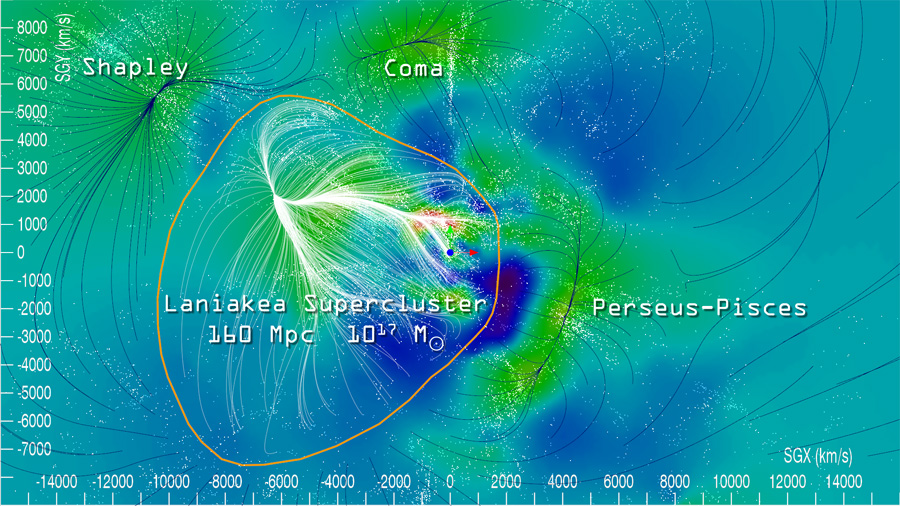
\includegraphics[width=450pt]{Laniakea.jpg}
    \caption{A cross section of Laniakea is shown in supergalactic coordinates where the velocity flows are shown as white lines. The density map is shown in color, where the green areas are denser than the blue areas, which correspond to voids. The blue dot corresponds to the Milky Way. This image of Laniakea is taken from the publication by Tully et al. (2014)\cite{tully_laniakea_2014} (Fig. 2) .}
    \label{fig:Laniakea}
\end{figure}

This supercluster is defined as a network of structures (formed by galaxies) that have convergent velocities towards a large attractor, shown in Figure \ref{fig:Laniakea}. This supercluster is called Laniakea. It has a mass of about $10^{17}$ Solar masses ($M_{\odot}$) and its semimajor axis has an approximate length of 160 Mpc \cite{NatureTully}.

Although modern astronomy has advanced considerably in the study of galaxy clusters \cite{TheDeepUniverse}, much is still unknown about the statistical properties of these superclusters. To get some answers in this topic it is necessary to use cosmological simulations.

\subsection{Cosmological simulations}
Obtaining direct experimental results in the study of cosmology is very complicated since they require observation times of billions of years and involve distances that light would take thousands of centuries to travel. Computational simulations in cosmology are powerful tools that allow us to study a great variety of events, from collisions of galaxies to the temporal evolution of  universes with different properties. All this thanks to algorithms that implement numerical solutions to physical theoretical models, such as particle phyics, hydrodynamics, N-body systems and astrophysics.
\begin{figure}[!h]
    \centering
    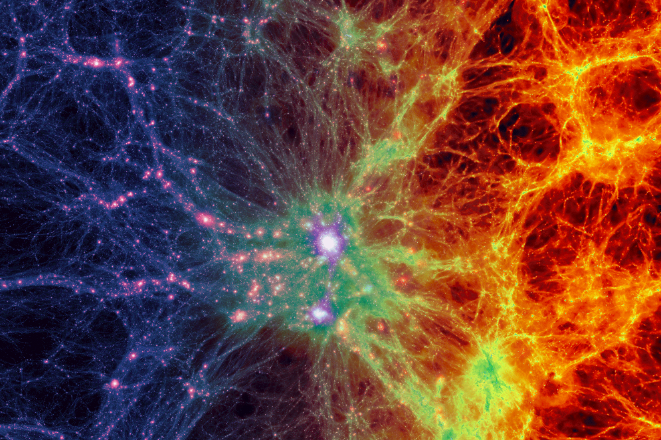
\includegraphics[width=450pt]{illustris.jpeg}
    \caption{This image was obtained by the Illustris Project \cite{IllustrisHome} and it is a cut of 15 Mpc $h^{-1}$ in thickness of the simulation when a time of 13.7 billion years has passed, which is the age that we believe our universe has. The dark matter concentration is shown to the left and the baryonic mass concentration is transitioned to the right.}
    \label{fig:illustris}
\end{figure}

Although different cosmologies can be simulated today on a large scale, most of the simulations that have been done use the standard cosmological model, or $\Lambda$-CDM model, which will be discussed more fully in section \ref{sec:units}.
Usually these simulations have as initial conditions a homogeneous space with particles of random mass with a certain distribution, and their evolution is dictated by gravitational interactions. Since mergers are usually allowed, it is expected that by the time of evolution of the system there will be compact objects that tend to form a large-scale structure, as you can see in Figure \ref{fig:illustris}. These compact objects can be stars, galaxies, haloes of dark matter or agglomerations of these.




\newpage
\section{Methods}

We describe below the methods to segregate superclusters in simulations.

\subsection{Grid Construction}


The cubic space of the simulation is segmented into a cubic grid. Each side of the box is divided into $N_{side}$ steps, dividing the three-dimensional space into $N_{side}^3$ equal voxels\footnote{In 2D dividing a surface in a grid with \texttt{n} steps  per dimension make $n^2$ squares of equal dimensions called \textbf{pixels}. In the 3D case, dividing a volume with \texttt{n} steps per dimension lead to the construction  of $n^3$ cubic Voxels. }. This in order to have a differentiable field that has already been quantized on a defined spatial scale, such as observational data.
 
\subsubsection{Velocity Grids}
\label{sec:INTROVgrid}
For each voxel we compute the \texttt{Center of Mass velocity}  

\begin{equation}
V_{CM_j}=\frac{\sum\limits_{i=1}^n m_i \textbf{v}_{i_j}}{\sum\limits_{i=1}^n m_i} \,,
\label{eq:CMcalc}
\end{equation}

Where \texttt{j} is the axis of interest, $m_i$ is the mass of the \textit{i-th} halo with speed $\textbf{v}_{i_j}$ along the axis \textt{j}. Once this is done, the result is a Three-Dimensional cubic Lattice with $N_{side}^3$ real numbers for each component of velocity. In 3 Dimensions, $V_x$, $V_y$, $V_z$ are grids of size [$N_{side} \times N_{side} \times N_{side}$] containing scalar numbers expressing the velocity component along the respective axis.

The number of steps $N_{side}$ is established from the beginning.
% but it is necessary to make a sensible choice. If $N_{side}$ is very large, the voxels are small. This is because the volume $V_{vox}$ of each voxel can be expressed as:
% \begin{equation}
%     V_{vox}=\frac{V_{Tot}}{N_{side}^3}
% \end{equation}
% Here, $V_{Tot}$ is the total volume of the space of the simulation. 

% The problem that the volume of each voxel is very small is that it decreases the amount of objects it contains, causing some voxels to be empty or with very few objects. This makes using the grid useless, since it does not increase the efficiency of the calculation nor does it take into account group properties between Halos.

% On the other hand, if $N_{side}$ is very small and the volume of the voxel is of a size considerably similar to the total volume, detail is lost in the spatial analysis of the velocities. It is advisable to adjust the number of voxels according to the size of the simulation, the detail that is desired in the spatial analysis and the computing capacity that is possessed.
% Since the simulations that will be used have already had certain time of evolution, it would be expected that some velocities of the voxels were aligned or even converging in some points.

% The grids have been built and each voxel corresponds a scalar number of speed in each of the three axes. Given these 3 components, the magnitude of the velocity for each voxel can be easily calculated.
% \begin{equation}
%     V_{mag_{ijk}}=\sqrt{V_{x_{ijk}}^2+V_{y_{ijk}}^2+V_{z_{ijk}}^2}
% \end{equation}
% The Grid $V_{mag}$ is the \textbf{Speed Grid} of the given Velocity spatial distribution. Remember that  $V_{x_{ijk}}$,$V_{y_{ijk}}$,
% $V_{z_{ijk}}$ are the scalar numbers corresponding to the velocity grids in X , Y and Z , respectively. $ V_{mag_{ijk}}$ is a \textit{positive} scalar corresponding to the speed of the center of mass of the voxel in the grid coordinates
% \texttt{i,j,k} expressed in \texttt{Km/s}.


\subsubsection{Mass Grid}
\label{sec:INTROMgrid}
In the initial conditions, each voxel has a bound mass corresponding to the total mass of the Halos inside the voxel. Let \texttt{M} be the \textbf{}{Mass grid} with side $N_{side}$ such that:
\begin{equation}
    M_{ijk}=\sum\limits_{n=1}^{\alpha} m_n 
\end{equation}

Where \textt{i}, \textt{j}, \textt{k} are the coordinates in the 3D grid of a given Voxel and $\alpha$ is the number of Halos contained in the volume described by the Voxel. 


\subsection{Gaussian Convolution}
\label{sec:INTROGCOnv}


To further highlight the group characteristics and to maintain an adequate theoretical framework, the mass and the velocity field on each axis is smoothed with a three-dimensional Gaussian convolution. For this Gaussian convolution process it is necessary to determine a $\sigma_{vox}$ given in voxels that determines the width of the 3D Gaussian curve. The larger the $\sigma_{vox}$ , the wider the curve and the interpolation loses detail. This $\sigma_{vox}$ can be set different for each axis but as there is not a peculiar direction or axis, it may be set equal for all three axis. This Gaussian filter which convolves with each three-dimensional array for velocities has the form:

\begin{equation}
    I_{i',j',k'}=\frac{1}{\sigma_{vox}^3 (2\pi)^{3/2}} \exp{ \left[ \frac{(i'-i_o)^2+(j'-j_o)^2+(k'-k_o)^2}{\sigma_{vox}^2}\right]}
\end{equation}

Where $I_{i,j,k}$ is the intensity of the Gaussian filter in the reciprocal lattice coordinates \texttt{i', j', k'}. In this case $i_o$, $j_o$, $k_o$ are the coordinates of the peak of the Gaussian filter.
 





\subsection{Velocity Divergence Coeficient (VDC)}
\label{sec:INTROVDC}
Supercluster identification studies Halo group velocities. Sometimes the convergence of speed in a local group of voxels can be seen at first sight as a group of speeds that point to a common center, but in a large part of the cases it is not so easy to show the formation of a supercluster . This is because in many cases a local group converges to a center whose own speed is different from zero and to the naked eye this group moves in a single direction without converging.

To determine which voxels are converging or diverging from certain centers, it is necessary to quantify the accretion for each unit of volume. This accretion is interpreted as the volumetric flow of velocity vectors for each voxel, in such a way that a scalar is assigned to each point of the three-dimensional grid.
%\subsubsection{VDC Grid}
The velocity divergence is calculated over a grid as:
\begin{equation}
\Phi_{i,j,k}=\frac{Vx_{i-1,j,k}-Vx_{i+1,j,k}+Vy_{i,j-1,k}-Vy_{i,j+1,k}+Vz_{i,j,k-1}-Vz_{i,j,k+1}}{\Delta h}
\label{eq:VDCcalculo}
\end{equation}
Where $\Delta h$ represents the volume differential evaluated.


This scalar $\Phi$ is called the \textbf{Velocity Divergence Coeficient} and, in this context,   quantifies the accretion in the grid.
% in such a way that those points where the velocities converge are assigned with a positive scalar and the points where it diverges acquire a negative scalar. In this order of ideas, the scalar is close to zero for those voxels where velocity only transits, does not converge or diverge. This means that when calculating this coeficient the effect of \textbf{transit formation} is taken into account. This refers to those regions where the speeds do not converge and tend to look like a transit region, but in fact if there is structure in formation with a certain speed regarding the frame of reference.
% Once the VDC has been calculated for each voxel in the grid, a new grid \textbf{$\Phi$} of dimensions  \texttt{[$N_{side}$ x $N_{side}$ x $N_{side}$]} is constructed and it contains the VDC scalars for each voxel in the grid.



\subsection{Watershed algorithm}
\label{sec:INTROWatershed}
 There are many problems in science associated with systems difficult to quantify geometrically, either because it is a continuous medium with indefinite limits or because it deals with volumes that are difficult to solve analytically due to their complexity. In the case of superclusters of galaxies, we are talking about volumes that are in a wide range distribution and of great complexity in terms of shape. 

 When you look at an image generated by a large-scale simulation of the universe, it is easy to identify points where matter is being concentrated. Recognize the structure present in one of these images at a glance is a task that can be easily approached by eye, but in science that is not enough.
To segment the divergence grid into regiones of converging halo flows we use the \textbf{Watershed Algorithm}.


% Suppose we have an \texttt{n}-dimensional scalar field with certain diffuse perturbations that are prominent over the noise of the field. If one wishes to know the form and the limits of the influence of these alterations, it is necessary to have an algorithm that can perceive the difference from region to region. Moreover, the method impemented is expected to work in any dimensionality and, if necessary, in periodic boundary conditions of the scalar field. One method that meets these parameters is the 
As defined by several sources \cite{DelaunayTessellations_Schaap} \cite{BeucherSegmetation}, the watershed algorithm is a method of segmenting images by regions or objects based on the mathematical morphology of the field to be analyzed. It was mentioned and used for the first time by Beucher and Lantuejeul\cite{BeucherWatershed1979} in 1979 in order to analyze images with objects whose limits were not defined.

The method is called \texttt{watershed} since it compares the field with a landscape\footnote{We speak of a landscape in the case of a scalar map in 2 dimensions, where at each point of a plane corresponds a scalar that would correspond analogously to the height in that position. However it should be mentioned that this analysis can be done in one or more dimensions.} that is flooded by rain, as explained by Platen et al.(2007)\cite{CosmicWatershedVoidDetection}, where the water begins to concentrate in the local minima, or valleys, and the puddles begin to grow from these initial concentrations filling their local well. If each puddle were filled with paint of a different color and the field was completely flooded, there would be borders between puddles as lines that define the border between different puddles. In a more practical sense, it would be possible to differentiate valleys by assigning to each point of the plane the color of the valley to which it belongs. Continuing in the analogy of the landscape, it would be expected that these borders that are formed between colors appear in the peaks of the mountains since they would be the last points of the map that would be flooded.

This analysis is equivalent to making a sweep from the lowest values of the scalar field to the highest,or viceversa, assigning to the lowest isolated points (or origins) an indicator that will propagate with the shape of the scalar field as the sweep reaches higher values. These indicators that will be assigned to each point of the field are called \textbf{group identifiers} and are assigned following certain rules according to specific cases.

% For example, if the assignment rule for each space point were to assume the group identifier of its closest origin, a \texttt{Voronoi map} would be constructed. In this particular case, we want a set of points in a three-dimensional space to have the same identifier if their velocities in space indicate that they eventually converge.

Using watershed to segregate bodies has many benefits that can be noticed without much effort, some mentioned by Platen et al. (2007) \cite{CosmicWatershedVoidDetection}.
\begin{itemize}
\item The algorithm works independently of the shape of the field and the perturbations that will be classified. Superclusters are expected to have a barely defined shape and a totally random volume, so using Watershed is a valid proposal.
\item Since the selection rules can be adjusted at will, it is easy to include in the algorithm periodic boundary conditions, which were used in the simulation. This will prevent those groups that are crossing one of the faces of the simulation box from being partially recognized or divided.
\item The method is designed to sweep the entire field, independent of its dimensionality. At the end of its execution every voxel in the space of the simulation would have assigned a group identifier. The field will be divided into different compact regions with defined borders and volumes.
\item The nature of the algorithm makes it more sensitive to field variations near the boundaries of each group. This is because at the borders the gradient of the field is weaker and any minimum fluctuation is relevant. Although the borders of the groups can not be clearly defined, the algorithm defines the borders of these diffuse objects very well.
\end{itemize}

\subsubsection{Selection rules and Parameter definition}
When talking about using this method, the selction rules that determine the identifiers of each voxel must be discussed. This problem is reduced to defining a selection criterion that is made from voxel to voxel while the sweeping by levels of watershed is carried out. 

To do this, the same neighborhood rule as in section \ref{sec:INTROVDC} will be used to assign the group identifier. We are talking about  a 6-connectivity, that means that only the 6 immediate neighbors of each voxel will be reviewed to establish the selection criteria when the watershed sweep passes through it. The cosniderations to use the method in this case are the following:
\begin{itemize}
    \item Once the VDC grid $\Phi$ has been calculated its minimum  and maximum value must be found\footnote{It is expected that the minimum value is a negative coefficient and the maximum value is a positive one, both of the same order of magnitude. This is easy to see in the VDC distributions shown in Figure \ref{fig:VCD_Varios}.}. These values are points of reference for doing the sweep in VDC values inside the grid. If you want to find the regions that correspond to structure formation , you will carry out the sweep from the highest values of VDC to the lowest ones. If what is desired is to find voids then the sweep should be made from the lowest values to the highest ones.
    
    \item Suppose that the sweep is first encountered with a voxel with coordinates \texttt{[i,j,k]} inside the grid and that has its corresponding value in the axial speed grids $V_{xyz}$, the mass grid \texttt{M} and , obviously, the VDC grid $\Phi$. In this point we must define a new variable called the \textbf{Tolerance Threshold Radius} $R_T$\footnote{This quantity is defined for the rest of the analysis. $R_T$ is the same for every instance of the watershed sweep.} for origins\footnote{the voxels classified as \textbf{Origin} are those that are the first to assume their identifier. They are those voxels from which the different regions propagate thanks to the method itself.}.  It is a discrete quantity that expresses the minimum number of voxels that must exist between two different origins. That is, if there is already an origin in a distance less than $R_T$ the current voxel can \textbf{NOT} be classified as an origin. Since the first peaks are within unclassified regions, most of these are classified as new origins. This measure is taken in order to prevent over-saturation of origins and poor classification of groups due to this problem.
    
    \item Now suppose that the sweep reaches another voxel with coordinates \texttt{[i,j,k]} inside the grid. This time the voxel is not isolated, but it is neighbor of a \texttt{single} voxel already classified. in that case the voxel assumes the identifier of its classified neighbor. If when the voxel is reached it has \texttt{more than one} classified neighbor, among these options the voxel assumes the identifier of the closest source. This allows that if the sweep is done properly, the region expands according to the shape of the scalar field. In addition, if the algorithm is in a dilemma to decide which identifier to assume for the current voxel, the nearest source can be selected because it is the accretion nucleus most likely to be linked to the voxel.
    \item The sweep is usually a narrow range that shifts between the two extreme values of VDC and all voxels with a VDC in this range range are evaluated. Unfortunately, the thinner this range is, the more computing time is required as more iterations are necessary to complete the sweep. This is why, although the range used is as narrow as possible, sometimes it is thick enough to evaluate more pixels of the account. Suppose that the voxel being evaluated is close enough to another origin and can not be classified as a new origin, but it does not have any classified neighbor either. In these cases the algorithm leaves this space unclassified.
    \item By the end of the sweep, many voxels in the grid will already have an identifier assigned. But it is not the case of all voxels; There are some voxels that the algorithm could not reach and therefore, they remained unclassified. One solution is to do the sweep again, this time a little thinner, in order to have a more sensitive evaluation interval for small VDC variations. However, this seems to just keep leaving some areas unclassified. This is why a lower weight variable called the \textbf{Qualification Threshold} ($Q_T$) is introduced. Represents the number of unsorted voxels that can be left in order to move to the \texttt{Final Assignment Stage}. This threshold is simply an indicator of when the method should stop doing watershed sweeps.
    \item \textbf{Final Assignment Stage .} When the number of unclassified voxels is equal to or less than $Q_T$, we proceed with a more robust classification. As mentioned before, it is valid to assume that in case of uncertainty about the identifier of a voxel, the logical thing to do is assign it the identifier of its closest source. This decision is also based on results obtained by Platen et al. (2007)\cite{CosmicWatershedVoidDetection} when it points out the similarity between the clusters obtained by the watershed method applied to velocities and those obtained by the Voronoi distance method. This selection by distance is carried out on the unclassified voxels. In this way, at the end of this step, all the voxels in the grid would have an assigned identifier.
\end{itemize}
Having said that, a good start is to define the parameters mentioned.

In order to choose an $R_T$ one should take into account the smoothing of the field. If the field was smoothed with a very small $\sigma_{Vox}$, a very large $R_T$ would be absurd since it would be assumed that the superclusters have diameters of the order of $R_T$. Assuming this is dangerous since by smoothing the field with a small $\sigma_{Vox}$ it was established that the smallest possible perturbations have diameters similar to $2 \sigma_{Vox}$. This would lead to a failure in the method so catastrophic that the established protocol would leave unsorted many voxels. It would be necessary to establish a very large $Q_T$ in order to be able to assign an identifier to each voxel. Doing this would make the segregation of groups more similar to the construction of a Voronoi map.

On the other hand, if the $\sigma_{Vox}$ is very large compared to $R_T$, then any sufficiently strong perturbation near a local accretion nucleus would be taken as a new origin. This leads to \texttt{over-saturation} of identifiers where the algorithm defines so many new groups that it results in an absurdity.

To avoid either of the two cases, it is sensible to evaluate what possibilities are available to choose $R_T$. Since defining $\sigma_{Vox}$  is establishing the \textit{minimum radius} that can have any disturbance in the VDC grid and assuming that all disturbances have said radius, the minimum possible distance between two accretion nuclei would be $2 \sigma_{Vox}$. That is why for the development of future methods that is the $R_T$ that will be chosen\footnote{ The  value asigned for $ \sigma_{Vox}$ is of 1 voxel for further analysis, then $R_T$ should be 2 voxels.}.
\begin{equation}
    R_T = \text{2 } \sigma_{Vox}
\end{equation}
Now, to choose $Q_T$ one must quantify the computational capacity that is possessed and the amount of uncertainty that is desired. Remember that the smaller $Q_T$ is, the more watershed sweeps must be done to assign indicators to sufficient voxels and reach the threshold. But if $Q_T$ is very large, the level of uncertainty increases since there would be a large percentage of voxel assigned by distance criterion and not by the watershed method. It is advisable to explore by trial and error the value of $Q_T$ and select one that meets the desired computational and uncertainty requirements. Since the voronoi method has a high degree of similarity with watershed, the relevance in terms of error of assigning a few voxels by distnance method is very low. For this particular case, a $Q_T$ according to the needs of this work is selected.

\begin{equation}
    Q_T = \text{200 Vox}
\end{equation}
Once the parameters to implement the watershed method have been defined, it is only necessary to use it on the appropriate VDC grid.In Section \ref{sec:Sigmainfluence} the influence of $\sigma_{Vox}$ on the characteristics of the superclusters found will be discussed in detail. On the other hand, Section \ref{sec:superclusterRecons} continues with the study of the case of a chosen  $\sigma_{Vox}$ having already applied the watershed algorithm in the respective VDC grid $\Phi$.

\subsubsection{Supercluster recosntruction}
\label{sec:superclusterRecons}
The best question that can be asked now is: \textit{what is the  $\sigma_{Vox}$ for making a reasonable comparison with the observational data?}

Notice that regardless of which $\sigma_{Vox}$ is suitable for future analysis, the other $\sigma_{Vox}$ also contain relevant information on large-scale structure formation. Using a different Gaussian smoothing does \texttt{NOT} skew or delete the original information, but it does give new information about the organization of the field at different scales. The right $\sigma_{Vox}$ is chosen according to how similar are the conditions of the superclusters found in the simulation and those that cosmologists and astronomers have observed in our galactic neighborhood. The first candidate is postulated inspired by the work of Tully et al.\cite{tully_laniakea_2014} and Platen et al. \cite{CosmicWatershedVoidDetection}. Both works coincide in that when looking for cosmological structures, such as superclusters or voids, it is sensible to do it for structures with diameters between 10 Mpc $h^{-1}$ and 100 Mpc $h^{-1}$ \footnote{These values are estimations that are proposed in this work. Platen looks for voids with proposed diameters between 20 Mpc $h^{-1}$ and 50 Mpc $h^{-1}$ , while Tully in his work on Laniakea calculates a semimajor axis for the local supercluster of 160 Mpc $h^{-1}$ .}. Defining a  $\sigma_{Vox}$ is indirectly defining the minimum radius that a disturbance of the scalar field can have. Given the above, for the rest of the characterization and comparison work this specific $\sigma_{Vox}$ will be used:
\begin{equation}
     \sigma_{Vox} = \text{1 Vox} = \text{10 Mpc }h^{-1}
\end{equation}





\subsection{Inertia and Geometric Properties}
\label{sec:IN}
For each supercluster we compute the following properties.
\paragraph{Center of Mass .} 
The positions of the centers of the voxels and the mass associated with each of them are known. We compute the center of mass as 
\begin{equation}
    CM_k = \frac{\sum\limits^{n}_{\text{j=1}} m_j k_j}{\sum\limits^{n}_{\text{j=1}} m_j} \,,
\end{equation}
where $CM_k$ is the coordinate of the CM along the \emph{k-th} axis of the simulation, $m_j$ is the mass of the voxel $j$ and $k_j$ is the \emph{k-th} coordinate of the voxel $j$. 


\paragraph{Intertia Tensor .}
Having the positions and magnitudes of the individual masses in a system also facilitates the calculation of the Inertia Tensor. This is no more than a mathematical representation that has information of moments of inertia associated with a rigid body. This second-rank tensor \textbf{I} is calculated from the moments of inertia associated with each coordinate axis and the inertia products. Note that  the distances $x_j$, $y_j$, $z_j$ are relative to the coordinates of the center of mass.

\[
  I=
  \left[ {\begin{array}{ccc}
   \sum\limits^{n}_{\text{j=1}} m_j (y_j^2 + z_j^2) & -\sum\limits^{n}_{\text{j=1}} m_j x_j y_j & -\sum\limits^{n}_{\text{j=1}} m_j x_j z_j  \\
   -\sum\limits^{n}_{\text{j=1}} m_j x_j y_j & \sum\limits^{n}_{\text{j=1}} m_j (x_j^2 + z_j^2) & -\sum\limits^{n}_{\text{j=1}} m_j y_j z_j  \\
   -\sum\limits^{n}_{\text{j=1}} m_j x_j z_j & -\sum\limits^{n}_{\text{j=1}} m_j y_j z_j & \sum\limits^{n}_{\text{j=1}} m_j (x_j^2 + y_j^2)  \\
  \end{array} } \right]
\]



\paragraph{Intertia Moment and Principal Axes of Rotation. }
The Inertia tensor contains information about the rotation properties of a rigid body, including the proper directions of rotation of the object and the moments of inertia associated with these axes. Speaking of the tensor \textbf{I} as a linear element, its eigenvectors and eigenvalues correspond to the directions of the main axes of rotation relative to the center of mass $\Vec{d}_k$ in the simulation coordinate sistem and to the associated moment of inertia $\lambda_k$, respectively.
Obtaining the value of the three $\lambda_a$, $\lambda_b$ and $\lambda_c$ that the tensor \textbf{I} has makes it possible to draw conclusions about the shape of the rigid object in question. For example, if the moments of inertia with respect to each principal axis are equal, then it is a sphere. This can be inferred from the fact that the object does not have a preferential axis of rotation.










\newpage

\section{Numerical Context}
%Some considerations to keep in mind about the development of this work.
% \subsection{Software, Permissions and Ethical considerations}
% The development of the investigation will be done entirely in open source software under the Licenses \textbf{MIT License} and \textbf{GNU General Public License}. We will be careful when citing the work or results of other people that we use. Since the work is developed in free software, special licenses for any software are not necessary. The code used to analyze the simulation data is in the \textbf{Github} Repository \cite{Repositorio}.
\subsection{Simulation data}
\label{sec:SIMDATA}
It is necessary to clarify that at no point the advance in time of the simulation is taken into account. The data used are static states of the simulation having already passed a sufficient time for gravity to have evolved the system .
The simulation analyzed\cite{SimData} in this case has the characteristics shown in the Table \ref{tab:InitCondInfo}. The border condition used is periodic, this means that, during the simulation, all the matter that comes out through a wall of the simulation cube of side 1200 Mpc $h^{-1}$  enters through the opposite wall.



\begin{table}[H]
    \centering
    \begin{tabular}{|c|c|}
    \hline
    
        \textbf{Side length} & 1200 Mpc $h^{-1}$ \\
        \textbf{Total Volume} & 1.73 x $10^9$ Mpc  $h^{-3}$\\
        \textbf{\# Halos} &  3 x $10^6$ Halos (Aprox.)\\
        \textbf{Smallest Halo Mass} & 1.84 x $10^{10} M_{\odot} h^{-1} $\\
        \textbf{Hubble} & 0.678\\
        $\Omega_L$ & 0.692885 \\
        $\Omega_o$ & 0.307115\\
        $\Omega_b$ & 0.221610\\
        
        
    \hline
    \end{tabular}
    \caption{Data extracted from the simulation data header. $\Omega_L$ corresponds to the Density of Dark Energy, $\Omega_b$ to the density of baryions and $\Omega_o$ to the density of Matter. Refer to Sections \ref{sec:units} and \ref{sec:initanalysis} for more information.}
    \label{tab:InitCondInfo}
\end{table}

\subsection{Cosmological Model and Measurement Units}
\label{sec:units}
In order to properly interpret the information in table \ref{tab:InitCondInfo} and to continue with future studies, it is necessary to define the frame of reference that will dictate the logic and metrics of the N-body simulation. The frame used in this case is the current Standard Cosmological Model which is known as \textbf{$\Lambda$-Cold Dark Matter Model}, or \textbf{$\Lambda$-CDM model}. 

The $\Lambda$-CDM model is that which we assume as true for physics at cosmological scales. It imposes Einstein's theory of relativity as the one that determines the dynamics and gravitational interactions on this scale. This model proposes an energy that explains the expansion of the universe that Hubble documented in 1936 \cite{Hubble}. This energy is associated with the cosmological constant \textbf{$\Lambda$} described by Einstein in the theory of General Relativity (hence its mention in the name of the model) and is believed that is present throughout the space. This energy is called \textbf{Dark energy} and to this day it is a complete mystery for science.

The expansion of the universe, according to modern cosmology, depends on a scale factor \textbf{a(t)} that is not constant in time, which indicates that the expansion is accelerated. Based on this scale factor, the \textbf{Hubble parameter (H)} is defined, which dictates how fast a certain amount of space is expanded and, therefore, the speed at which two distant points move away.
\begin{equation}
    H = \frac{\dot{a}}{a}
\end{equation}
When we talk about the Hubble parameter for objects that are located in our galactic neighborhood, we find that it is a constant, defined as the Hubble constant \textbf{$H_o$}.
\begin{equation}
    H_o = \text{100 h km }s^{-1}  Mpc^{-1} = 67 \pm 7\text{ km } s^{-1}Mpc^{-1}
\end{equation}
Where \texttt{Mpc} corresponds to the unit of length measurement \emph{Megaparsec}\footnote{1 Mpc = $10^6$ pc = 3.087\text{ x }$10^{22}$ m.}. \texttt{h} is an adimensional constant defined with the Hubble constant.
\begin{equation}
    h \simeq 0.67
\end{equation}
Based on this, the simulation metric is defined. Note that the distances of the simulation come in terms of Mpc  $h^{-1}$ and not Mpc and, since the rest of the work will be done in units of Mpc $h^{-1}$, it is necessary to define the parameter \texttt{h} for the simulation, shown in table \ref{tab:InitCondInfo}.

\textbf{Remember} that Tully defined the length of the semimajor axis and the mass for Laniakea in units of Mpc and $M_{\odot}$, respectively\cite{tully_laniakea_2014}. However, in order to make comparisons, these measurements must be renormalized on this parameter \texttt{h} and thus be defined in the framework of the simulation.

The part of the title that talks about \emph{Cold Dark Matter} has two important concepts to deal with. The first is \textbf{Dark Matter}, which refers to an hypothetic unknown type of matter that arises conceptually to explain anomalous rotation speeds in galaxies and the formation of them\cite{GalaxyDM}. Dark matter does not interact with light or the rest of the electromagnetic spectrum (That is why it is obscure), but by definition it interacts gravitationally with itself and with baryonic matter. The second concept is the assertion that dark matter is \emph{cold}, which refers to the speed of movement of particles of dark matter does not reach relativistic limits.

This model then proposes three fundamental components for the universe and its behavior as a thermodynamic, isotropic and homogeneous system on a large scale. These three constituents are: matter, which includes dark matter and baryonic matter. dark energy and radiation, which groups electromagnetic radiation and neutrinos for their ability to move at relativistic speeds.

This model then proposes three fundamental components for the universe and its behavior as a thermodynamic, isotropic and homogeneous system on a large scale\cite{CARROLL}. These three constituents, expressed as abundances with percentage density parameters, are: \textbf{Matter} (\textbf{$\Omega_O$}), which includes \texttt{Dark Matter} (\textbf{$\Omega_c$}) and \texttt{Baryonic Matter} (\textbf{$\Omega_b$}), \textbf{Dark energy} (\textbf{$\Omega_L$}) and \textbf{Radiation} (\textbf{$\Omega_R$}), which groups electromagnetic radiation and neutrinos for their ability to move at relativistic speeds. The abundance of radiation is so small compared to the other two that it is omitted many times when establishing the parameters of a simulation  (\textbf{$\Omega_R = 0$}). The total percentage density $\Omega_T$ is equal to one and is expressed as $\Omega_T = \Omega_O + \Omega_R + \Omega_L = 1$. Remember that $\Omega_b + \Omega_c = \Omega_O$. 

\newpage
\section{Results}
In this section will be presented the results of applying the methods suggested above to an N-body simulation. 

\subsection{Grid construction}
Once the data of position, speed and mass of each object have been loaded, the construction of the grid is carried out. Since it is a cubic space with 1200 Mpc $h^{-1}$ per side, a good proposal for $N_{side}$ is 120. In this way each voxel would have a volume of $10^3 Mpc^{3}h^{-3}$ and there would be a total of 1,728,000 voxels in the whole space. 

\paragraph{Mass Grid.} The initial mass grid \textbf{M} is built with the method shown in \ref{sec:INTROMgrid}.
\paragraph{Velocity Grids.} Axial velocity grids \textbf{$V_{x}$} , \textbf{$V_{y}$} and \textbf{$V_{z}$} are build initially with a simple sweep of all the cells in the grid and using on each voxel the methods shown in Section \ref{sec:INTROVgrid}. \textbf{$V_{mag}$} is built as well based on the Axial velocity grids previously generated.  



\paragraph{Remember} that all of this grids has dimensions \texttt{[120 x 120 x 120]} since is the grid size used. each Voxel is [$10 Mpc h^{-1}$ x $10 Mpc h^{-1}$ x $10 Mpc h^{-1}$ ] in dimensions and has a volume of $10^3 Mpc^{3}h^{-3}$.

\subsection{Initial analysis}
\label{sec:initanalysis}
Since the whole simulation box volume is 17.28 x $10^{8} Mpc^{3}h^{-3}$ and the sum of every voxel in the mass grid \footnote{Notice this expresses the whole mass of the simulation box.} is 3.07 x $10^{19} M_{\odot}$, the \textbf{Universe Density of the Simulation} ,defined as the density of the whole simulation box, takes a value of:
\begin{equation}
    \rho_{s} = 1.78\text{ x }10^{10} M_{\odot} Mpc^{-3} h^{2}
\label{eq:UNI}
\end{equation}
\subsubsection{Initial Speed and Mass Distribution}


Once this new scalar for speed is calculated for each voxel in the initial condition, a distribution can be formed from counting the  speeds of all the voxels as shown in Figure \ref{fig:SpeedDistribution}. The Mass distribution of the simulation corresponding to the initial conditions is shown in Figure \ref{fig:InMassDistribution}. This is the \textbf{Initial Mass Distribution} of the simulation. 

This is \texttt{NOT} the distribution of mass that would be used later in the development of the characterization, as will be shown later, mainly because for future analysis it is necessary that the field of mass is differentiable.


\begin{figure}[h]
    \centering
    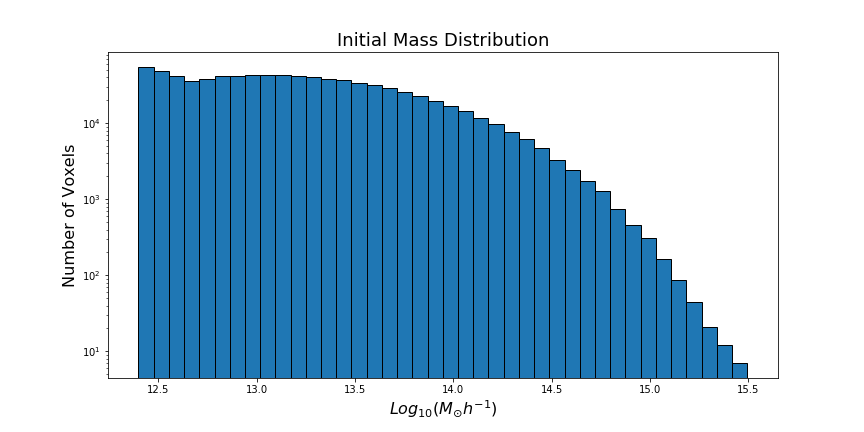
\includegraphics[width=\linewidth]{MD_0.png}
    \caption{Here is shown the mass distribution of all the \textbf{1'728,000 voxels} in the simulation box. The X-axis has a logaritmic scale of the mass for voxels expressed in solar masees. Here no filter has been applied.}
    \label{fig:InMassDistribution}
\end{figure}




  

\subsubsection{Quantifying Initial acretion with the VDC} \label{sec:VDCquantifyingResults}
Since the main purpose of using velocities to analyze the system is to quantify the accretion of different areas of space, it is necessary to determine this volumetric divergence of velocity for each voxel. For this the equation \ref{eq:VDCcalculo} is used. The VDC is calculated and, again, there is a distribution associated with the count of the VDCs of each voxel.

\begin{figure}[!h]
    \centering
    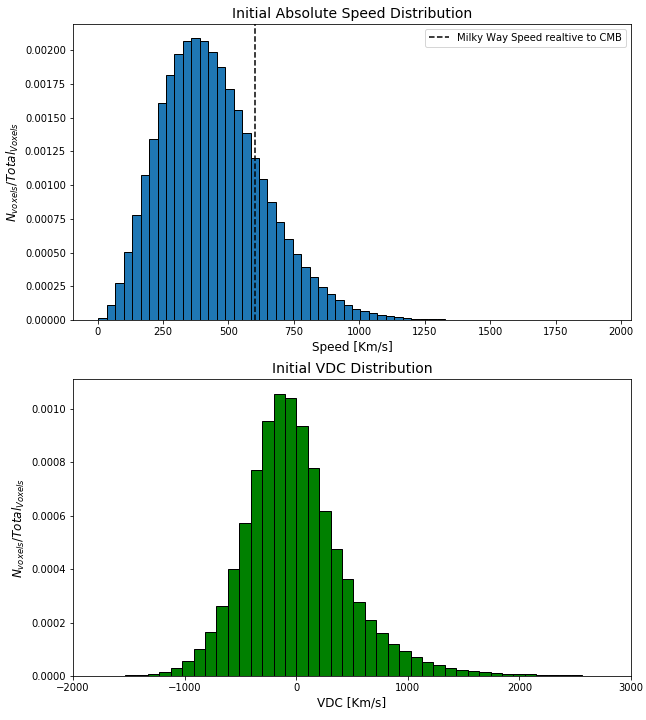
\includegraphics[width=320pt]{V_VDC_0.png}
    \caption{ The \textit{upper Histogram} shows the Initial distribution for the speed magnitude of every Voxel. The Speed of the milky way relative to the Cosmic Microwave Background is marked with a black dashed line, corresponding to 631 $\pm$  20 Km/s . The \textit{lower Histogram} shows the Initial VDC coeficient distribution along the voxels of the grid. This analysis is done without making any Gaussian filter over the speed fields.}
    \label{fig:SpeedDistribution}
\end{figure}

Since regions of high accretion are those in which matter is coming together, this matter must come from somewhere. That is why it is expected that there are regions where the accretion is negative, that is, where the haloes are moving away from each other. This can be seen in Figure \ref{fig:2D_VDC} where the zones with divergent velocity vectors have a negative VDC, while the regions where the accretion is large have a positive VDC.
It is expected that there will be almost the same proportion of positive and negative accretions since the simulation was carried out under periodic conditions and without external influence. There is a general increase of accretion when it comes to a gravitational model due to the large structure formation. Since gravity follows the law of the square inverse, it is expected that what is near the accretion nuclei is falling faster towards them than the matter that is close to the voids. That is to say that the areas that are attracting matter are filled at a higher rate than with which the voids are emptied. Given this, the values of positive accretion should be larger in magnitude than those of negative accretion.

\begin{figure}
    \centering
    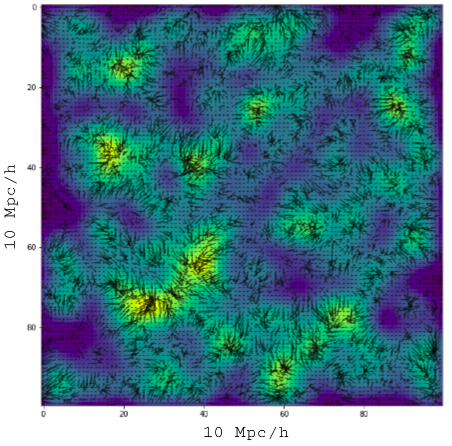
\includegraphics[width=320pt]{gauss.png}
    \caption{In a cross section of the 3D grid at a random Z, the corresponding  velocity vectors in X and Y are shown in black. The VDC field is shown in colors, where yellow zones have a big positive VDC and dark blue regions are those with big negative values for VDC. Notice how in these structures the VDC is much more positive in the center of the agglomerations than in the rest of the structure.}
    \label{fig:2D_VDC}
\end{figure}

Assuming there is a structure forming by a group of voxels, note that at no time the peculiar speed of the group itself is neglected. This is because it takes into account the difference between the incoming and outgoing velocities of each voxel and not the velocities themselves. For example, assume that there is a group of voxels that are close to each other with similar speeds in the same direction. At first glance, one could say that it is a transit region and that there is no structure in formation there. But when looking at the $\Phi$ grid, it may be noted that voxels have higher VDC towards the center of the studied region, which would mean that a structure is being formed and that its own velocity with respect to the inertial frame of the simulation is different from zero .


\subsection{Gaussian Convolution and Sigma relevance}

In his study about Laniakea, Tully\cite{tully_laniakea_2014} emphasizes a simple idea but with great influence on the study that will be developed. In his study is mentioned that, in cosmological frameworks, it is assumed that large-scale structure formation is due to Gaussian primordial fluctuations of the field of gravity. It is expected that as long as the density and speed fields evolution remain in the linear regime, they will keep their Gaussian properites. That is why to obtain adequate results it is necessary to take into account these Gaussian behavior of velocity and mass fields by smoothing them.
\begin{figure}[!h]
    \centering
    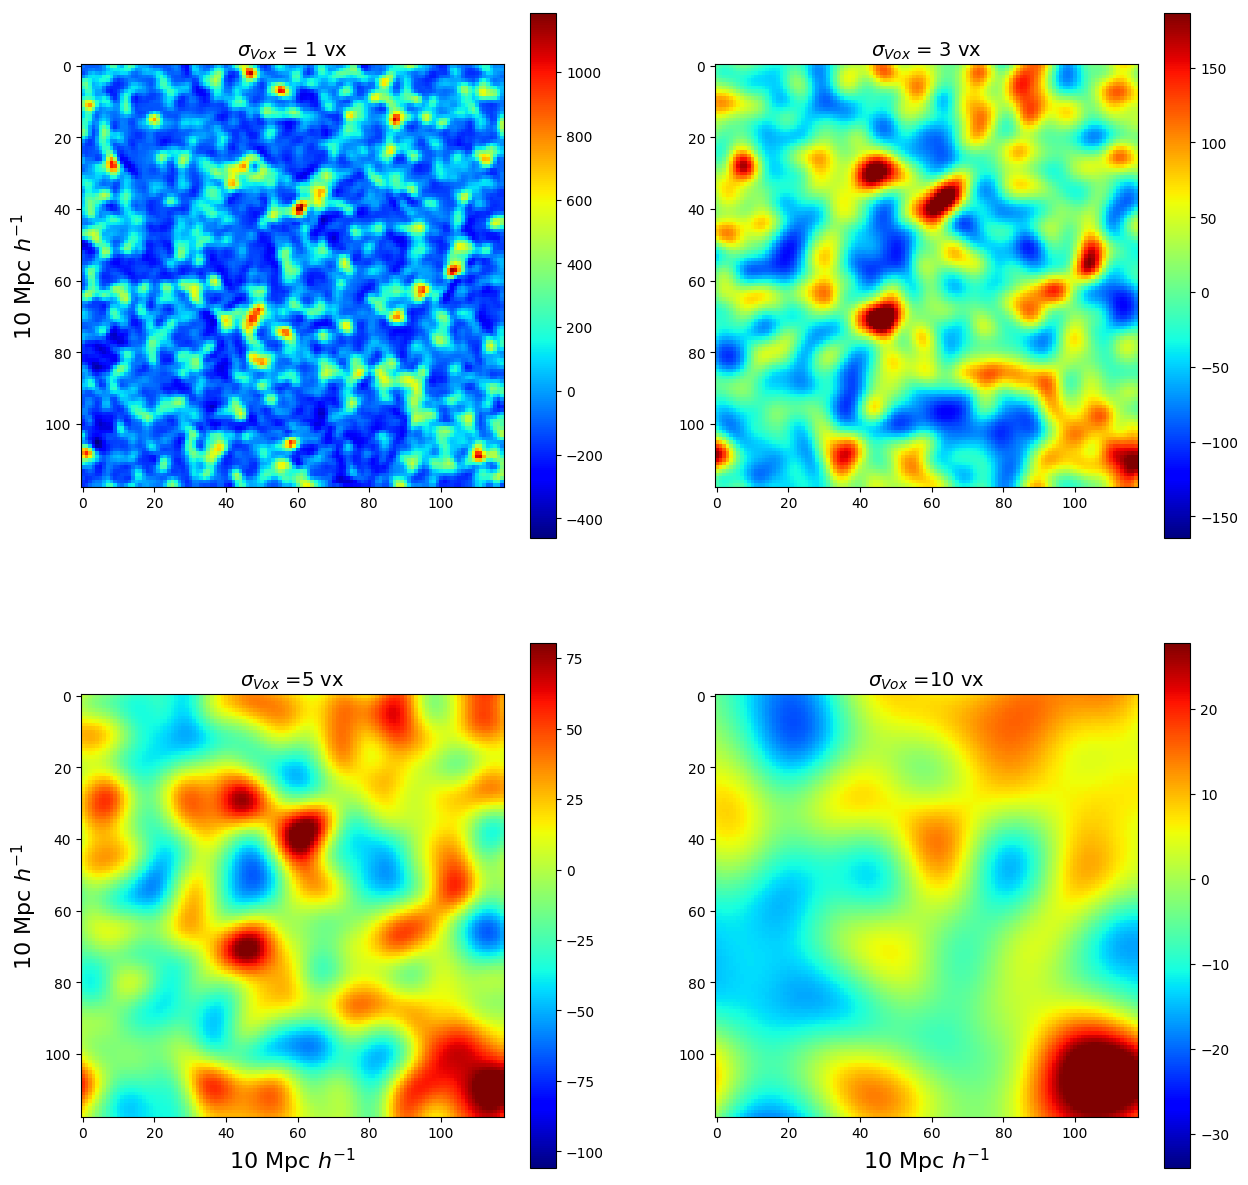
\includegraphics[width=380pt]{SigmasVDC.png}
    \caption{Here is shown  a random cross section of the softened VDC fields. The $\sigma_{Vox}$ used for every case is shown on top of every plot. Notice how peak values decrease while $\sigma_{Vox}$ value increases.}
    \label{fig:SigmasVDCZcut}
\end{figure}
Also, in order to perform the watershed analysis in a VDC grid it is necesary that the scalar field represented by the grid is differentiable, otherwise the watershed algorithm will find discontinuities and eventually will lead to the misclassification of superclusters.

In order to perform a complete watershed analysis over the VDC and extend it to characterization of superclusters based on features as volume or mass,  it is necesary to apply the  \textbf{same} Gaussian Filter to the 3D axial velocity grids and the mass grid as well. This in order to have consistent measures despite the smoothing of the VDC field.



\begin{figure}[!h]
    \centering
    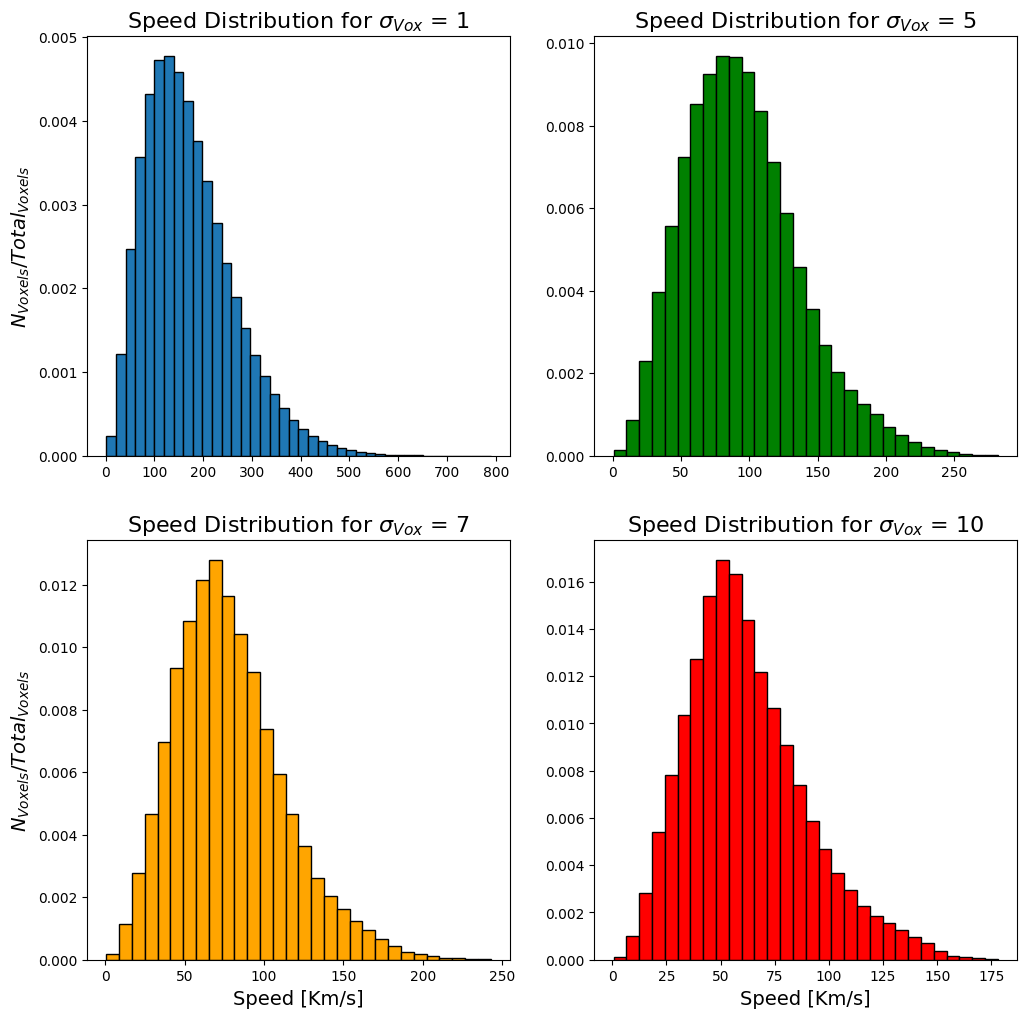
\includegraphics[width=400pt]{VMD_varios.png}
    \caption{A distribution of the speed magnitude for the voxels in the grid $V_{mag}$ calculated for different values of $\sigma_{Vox}$. Notice how the ranges of values change when $\sigma_{Vox}$ changes.}
    \label{fig:MD_Varios}
\end{figure}

To perform the smoothing, a $\sigma_{Vox}$ value is needed in order to define the width of the Gaussian Filter. With small $\sigma_{Vox}$\footnote{Small $\sigma$ are between 1 and 5 voxels in the grid reference. Big $\sigma$ are values of 15 voxels or more.} many structures are visible in a fine and defined network in the VDC grid, while big $\sigma_{Vox}$ only diferentiate big structures with barely any resolution of smaller filaments. Also, using big $\sigma_{Vox}$ cause peak values to be smoothed and values of the field \textit{move }closer to  the average value of the field. This effects can be seen in Figure \ref{fig:SigmasVDCZcut} where the same cross-section of the VDC grid is shown but smoothed with different values of $\sigma_{Vox}$.


\begin{figure}[!h]
    \centering
    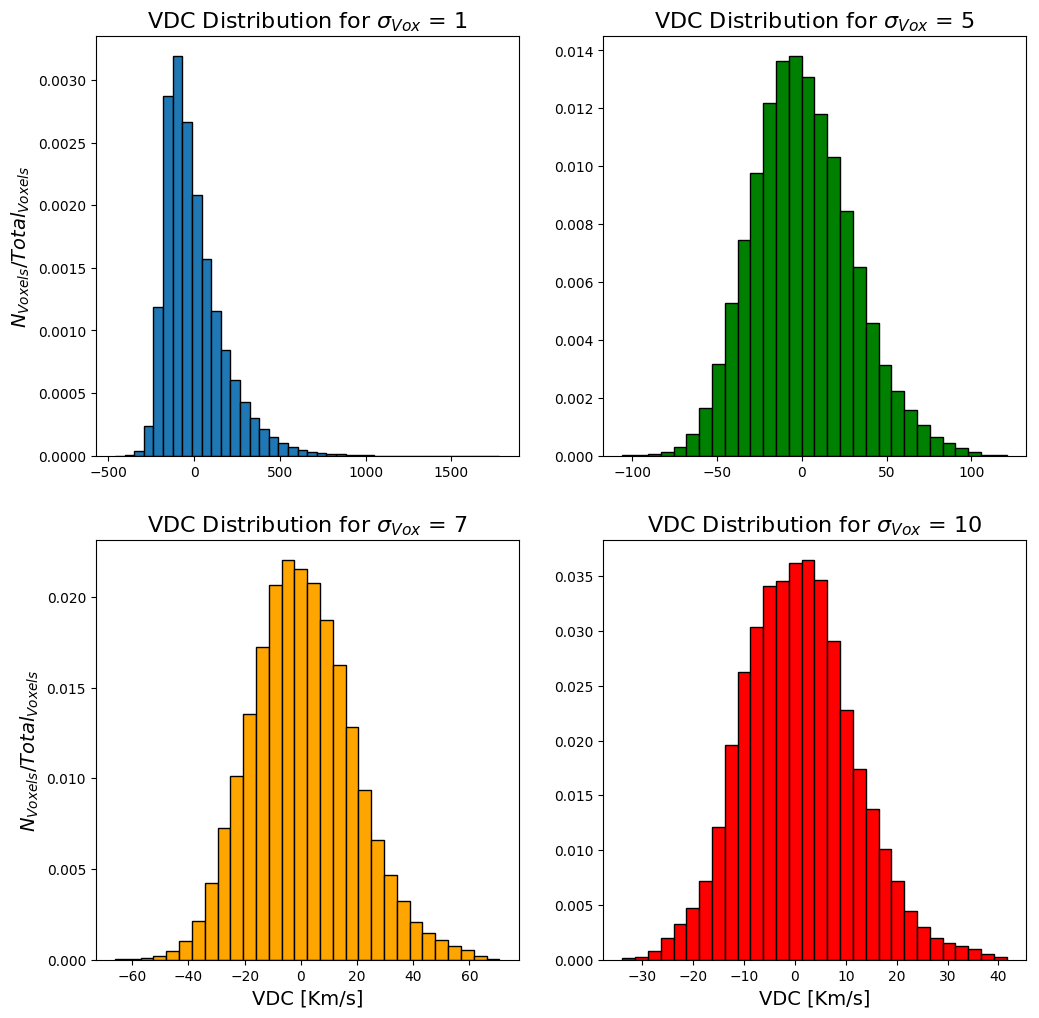
\includegraphics[width=400pt]{VCD_varios.png}
    \caption{A distribution of the VDC for the voxels in the grid calculated for different values of $\sigma_{Vox}$. Notice how the distibution ranges and expected values change when $\sigma_{Vox}$ changes.}
    \label{fig:VCD_Varios}
\end{figure}


\paragraph{Remember}  that once the $\sigma_{Vox}$ value has been chosen, the smoothing must be done for the axial velocity grids $V_x$, $V_y$, $V_z$ and the mass grid \textbf{M}. This in order to have coherent results in future processes.




Once the grids have been smoothed with a defined $\sigma_{Vox}$, it is evident that the magnitude of the values in the grids and the ones subsequently calculated is reduced. It was expected that this attenuation would happen since the interpolation brings the data closer to the field average. This can be evidenced in the figures \ref{fig:MD_Varios} and \ref{fig:VCD_Varios}.





% \subsection{Watershed Algorithm implementation and Region segregation}
 Hence in order to define geometric boundaries for random objects a powerful tool called  the \textbf{Watershed Algorithm} is used. For this problem the watershed method is fundamental for the recognition of clusters and, therefore, it is the backbone of this work.

% In section \ref{sec:INTROWatershed} the nature of the algorithm and its not-so-profound complexity are discussed. It is easy to intuit that this method will be applied to the VDC grid $\Phi$ since it is the only grid with enough information\footnote{The grid of mass \textbf{M} also provides information about large-scale structure formation, but leaves aside the information of the voids since their absence of mass makes it difficult to know where it converges.} to dictate whether a group of voxels is converging to a certain structure or are simply disconnected from each other as explained in section \ref{sec:VDCquantifyingResults}.



If the algorithm works properly, the regions that the algorithm segregates should be able to be compared at a glance with the perturbations of the VDC field. This can be seen in Figure \ref{fig:1Pert}, where a section of the smoothed scalar field with $\sigma_{Vox} = 1$ Vox and its respective classification is shown. Figure \ref{fig:3Pert} shows the same cut of the grid, this time smoothed with $\sigma_{Vox} = 3$ Vox, where it is easy to notice that in this last case the regions found are larger.

\begin{figure}
    \centering
    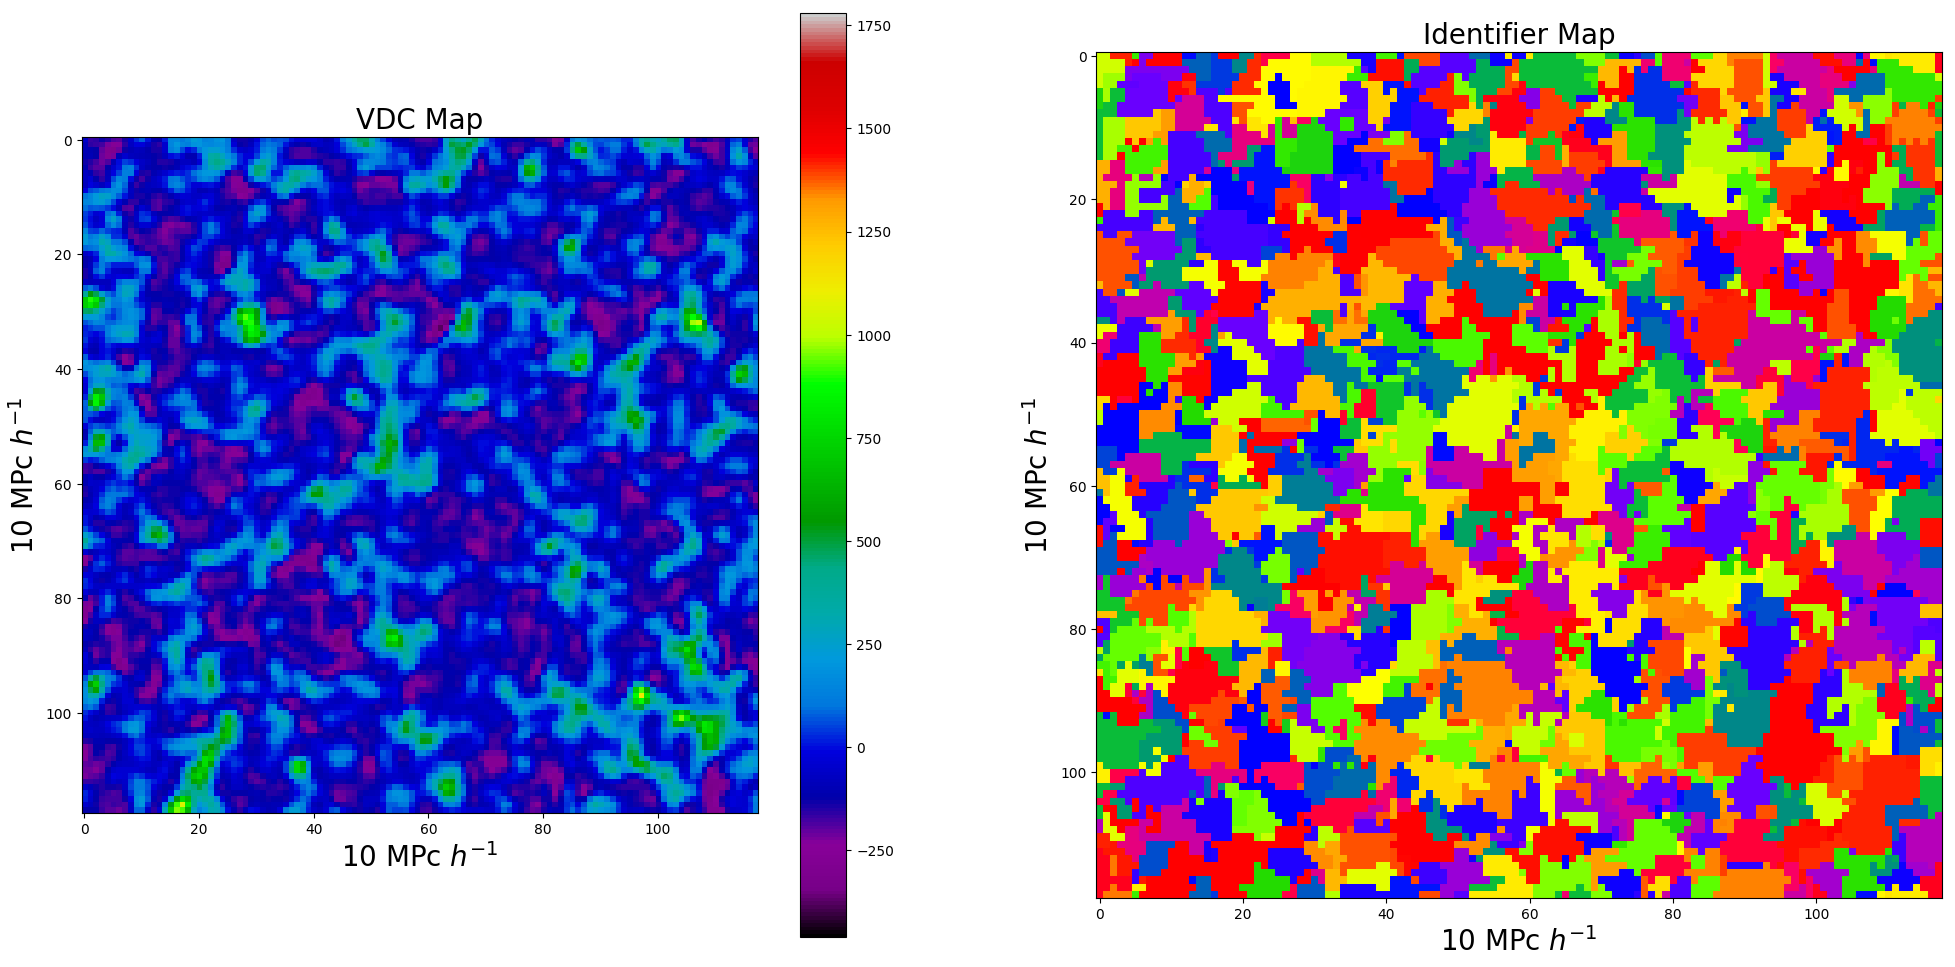
\includegraphics[width=380pt]{1PlotPert_48.png}
    \caption{On the left there is a random cut on the axis where the regions with different accretion are observed. On the right is the classification made by the Watershed method, where different regions have different colors.}
    \label{fig:1Pert}
\end{figure}

\begin{figure}[!h]
    \centering
    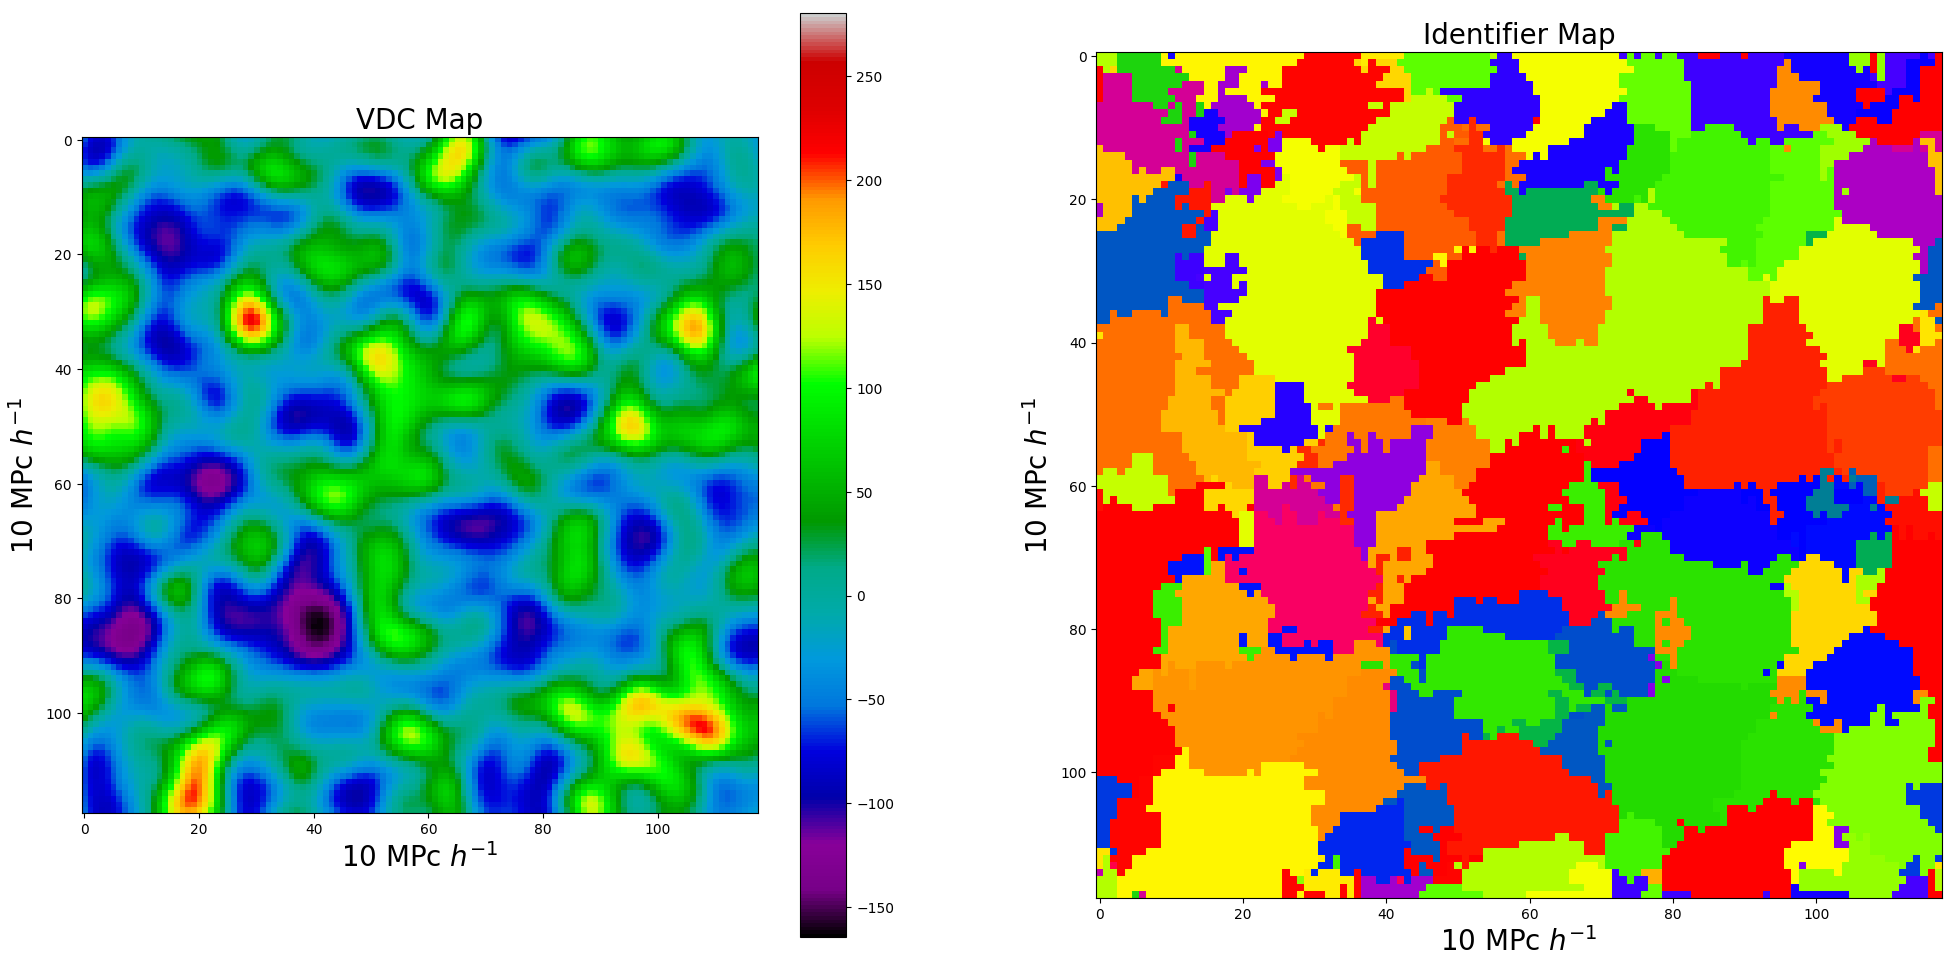
\includegraphics[width=380pt]{3PlotPert_48.png}
    \caption{This graph shows the same cross section as Figure \ref{fig:1Pert}, but this time the field was smoothed with $\sigma_{Vox}$. In this case, we can observe a vacuum structure represented in black, where the borders of several regions effectively meet. In both graphs it is seen how the distinguishable accretion peaks are classified as independent regions by the algorithm.}
    \label{fig:3Pert}
\end{figure}
As for the shape of the regions, superclusters are expected to have random and therefore unpredictable forms. However, it is possible to establish patterns that the regions must follow to determine if the algorithm is faulty or inefficient. For example, it is expected that in regions of void, i.e. those with negative accretion, the borders of many regions will be brought together. This is because they are the last parts of the scalar map that the surveyed of watershed evaluates. Figure \ref{fig:3Pert} shows a huge void where this predicate can be corroborated.


To visualize the behavior of the algorithm, it is applied on a grid already smoothed with a large $\sigma_{Vox}$. This is so that the structures are differentiable and can be compared with their respective allocation by regions. In this case $\sigma_{Vox} = 3$ vox is selected since it allows to have many superclusters in the space of the simulation with a large variety of sizes. In order to avoid plotting each point of the grid and visualize the main structures, it is convenient to plot those regions whose VDC values exceed a certain threshold. The result of this process is shown in Figure \ref{fig:3STRUCTURES}.
\begin{figure}[!h]
    \centering
    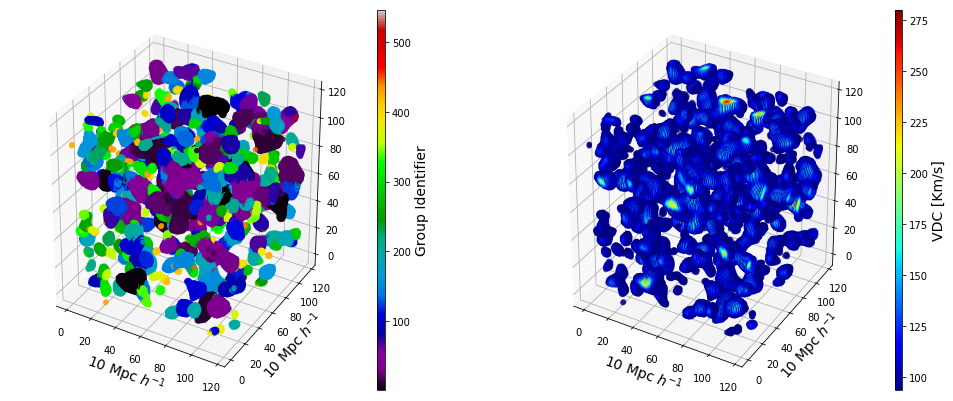
\includegraphics[width=450pt]{N65SegmentationSigmas137.png}
    \caption{The Watershed Algorithm with the parameters selected is applied the VDC Grid $\Phi$ for a field smoothed with $\sigma_{Vox} = 3$ Vox. On the right are shown those regions of the VDC field that exceed the threshold set at 0.65 $\Phi_{max}$, where $\Phi_{max}$ is the largest accretion registered in the VDC field $\Phi$. On the left is the classification by groups that the algorithm made for these same regions.}
    \label{fig:3STRUCTURES}
\end{figure}

The algorithm assigns an integer as the identifier for each voxel that the sweep evaluates. This integer is in ascending order, for simplicity of the algorithm. For example, the identifier \texttt{'1'} was assigned to the group associated with the \texttt{first} seed that was found, the identifier \texttt{'255'} was assigned to the group of the \texttt{255th} seed and so on. As expected, the first groups that the algorithm recognizes are those whose origin had very high accretion. These high accretion centers belong to the largest superclusters, which are expected to have the lowest identifiers.

\subsubsection{Sigma Influence Analysis}
\label{sec:Sigmainfluence}
Watershed's algorithm was performed on the grid $\Phi$ that was built with smoothed speeds $V_{xyz}$ with certain  $\sigma_{Vox}$. The method found a determined number of superclusters in the entire space and assigns each supercluster a group identifier. If the method was used, it is worth saying that all the points in the grid already belong to a group.

\begin{figure}[!h]
    \centering
    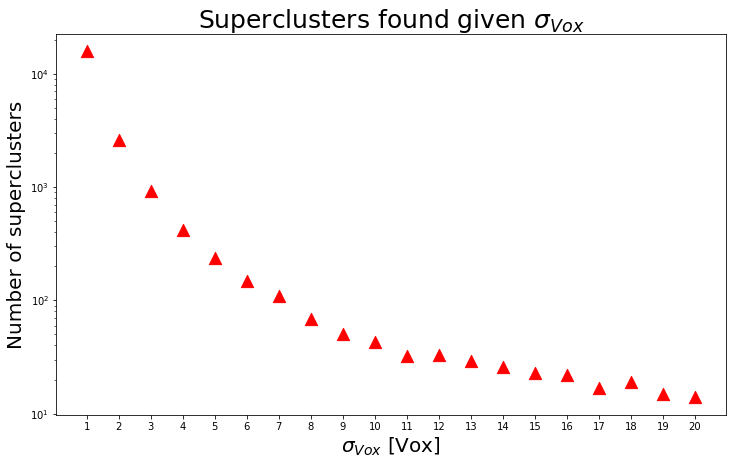
\includegraphics[width=320pt]{Nclusters.png}
    \caption{Here is shown that effectively a smaller $\sigma_{Vox}$ implies recognizing many more structures; This is because each structure is of a smaller volume and a larger quantity is required to fill the entire space of the simulation. In this case 15778 superclusters were obtained for $\sigma_{Vox}=1$ Vox, however for $\sigma_{Vox}=20$ Vox only 14 superclusters were identified.}
    \label{fig:Nclusters}
\end{figure}

When defining different $\sigma_{Vox}$, it is expected that prominent fluctuations in the VDC field occupy a greater or lesser volume depending on the chosen $\sigma_{Vox}$. Similarly, i't is expected that by using a larger $\sigma_{Vox}$, for example, the method classify superclusters that are larger and therefore more massive. Figure \ref{fig:Nclusters} shows the number of superclusters classified for each $\sigma_{Vox}$, while Figure \ref{fig:masaAcumulada}  shows a mass distribution with the number of superclusters with a mass equal to or less than a certain value. In both plots it is observed that the $\sigma_{Vox}$ is indeed relevant in the definition of large scale strutures in simulations.

\begin{figure}[!h]
    \centering
    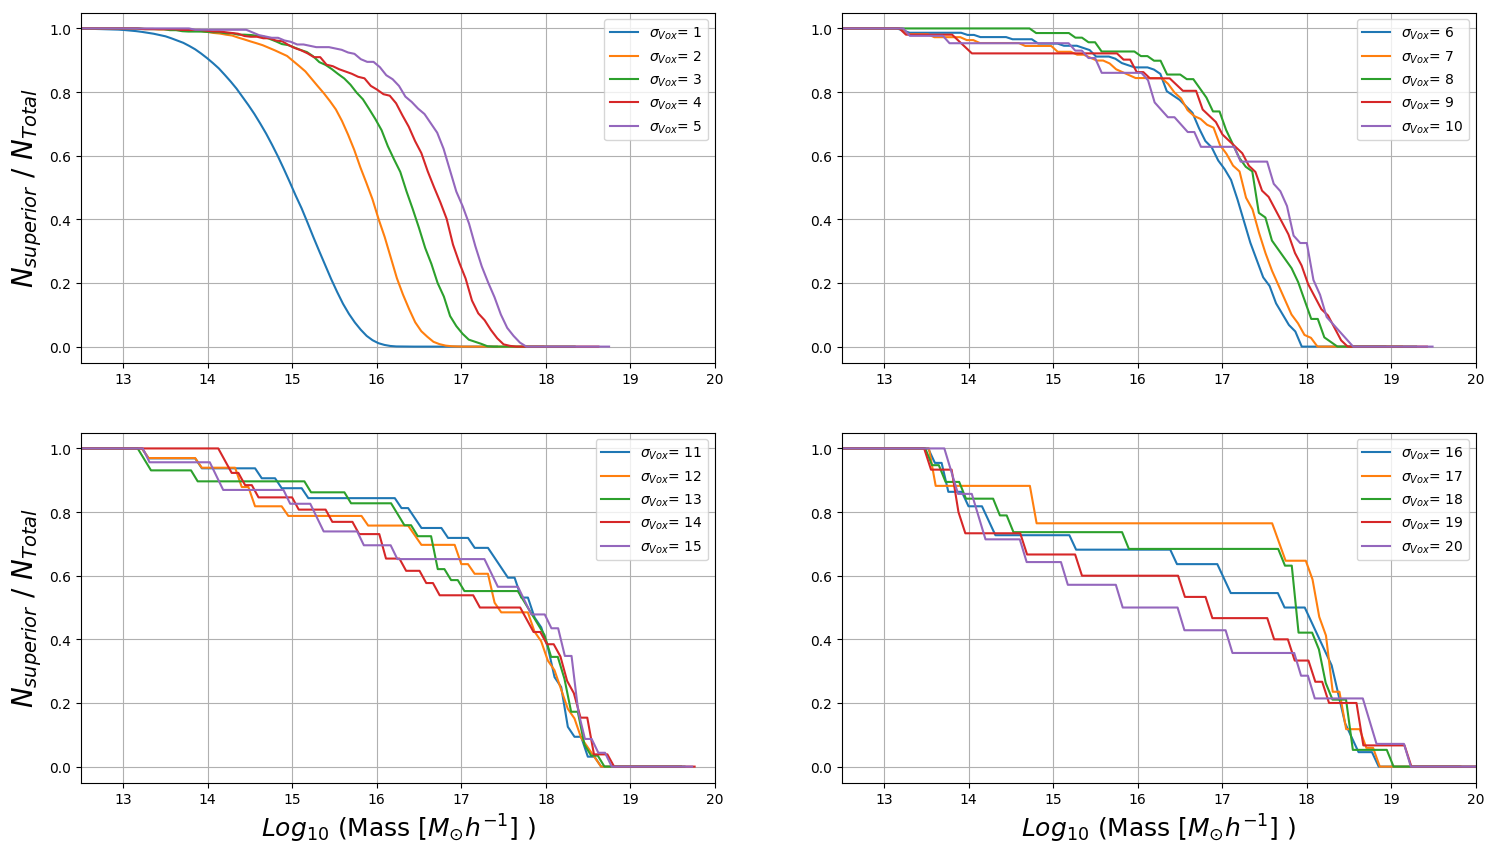
\includegraphics[width=420pt]{MasasMayoresnormc.png}
    \caption{Here we show the number of superclusters with masses above a certain threshold for each $\sigma_{Vox}$. As expected, applying the Gaussian filter with small $\sigma_{Vox}$ causes many small structures to be recognized, while using large $\sigma_{Vox}$ builds fewer superclusters but with much larger masses.}
    \label{fig:masaAcumulada}
\end{figure}

\subsection{Supercluster characterization}

On the VDC grid $\Phi$, the watershed scan with $\sigma_{Vox} = 1$ Vox is executed and \textbf{15778 superclusters} are obtained. As expected, the borders are not smooth and it is a varied \emph{Zoo} of shapes and sizes. Now we have a catalog of superclusters in the simulation, with definite volumes in the grid and, therefore, with a mass that is also defined. Each voxel already belongs to a group as well as the mass it contains and it is easy to extract new information from mass and volume statistics. By extension, these data also allow conclusions to be drawn about density. We also have spatial data of each voxel that belongs to each group. This is important since not only do you have the volume data, but you also know the shape of each supercluster. 

\begin{figure}[!h]
    \centering
    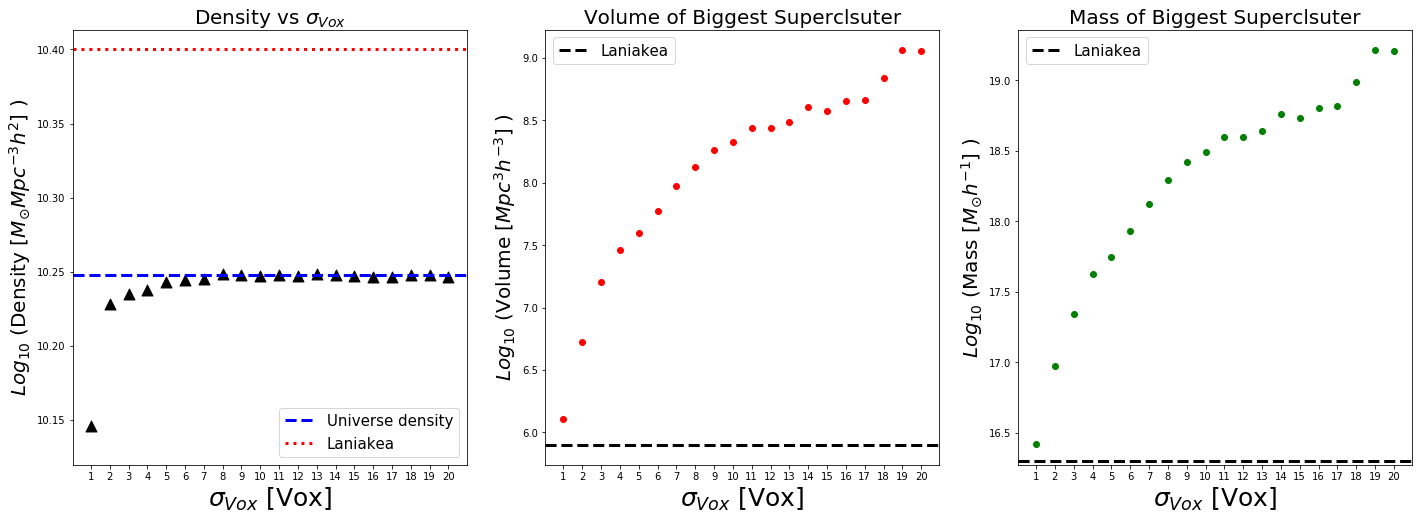
\includegraphics[width=450pt]{DensidadSigma.png}
    \caption{On the left, the average density of supercumulus is plotted for each $\sigma_{Vox}$. In the center and on the right, the largest volume and mass found for a supercluster are shown respectively. It is wise to clarify that the supercluster with more volume does not have to be the most massive.}
    \label{fig:DensMassVolLani}
\end{figure}

In this section the statistical analysis will be treated by these two flanks: on the one hand there is information on mass and density analysis, and on the other hand everything that has to do with the geometrical properties of superclusters.

\subsubsection{Mass, Volume and density}

The statistical data found on the mass and volume of the characterized regions make it possible to extrapolate their density easily since it is the ratio between these two values. In Figure \ref{fig:HISTVMD1} you can see a distribution for each of these three quantities, along with a density distribution\footnote{Redundancy intended} on these two axes. There is not only information about the simulation, but also the position of Laniakea in these distributions.

\begin{figure}
    \centering
    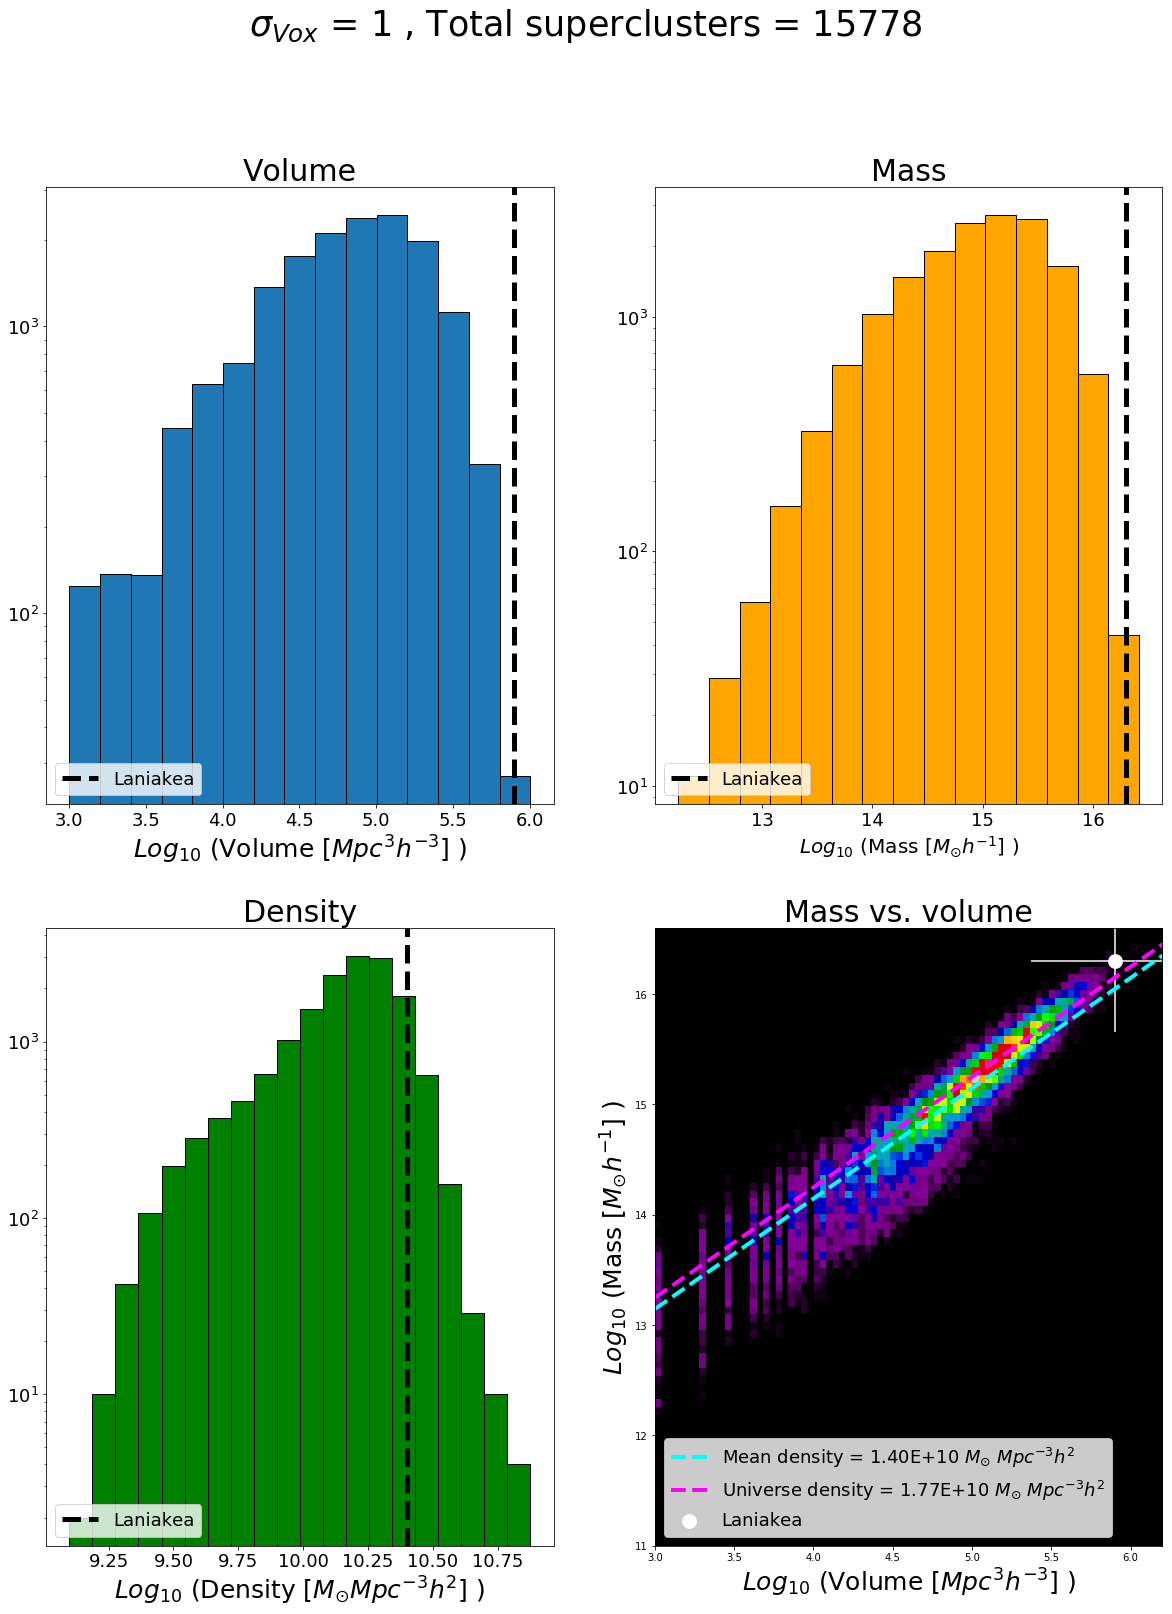
\includegraphics[width=360pt]{HistVMD_1.png}
    \caption{Distributions of mass, volume and density for the 15778 superclusters found with $\sigma_{Vox} = 1 $ Vox. Notice how, even with errorbars, Laniakea is at the edges of the distributions and in an atypical region of the density histogram. }
    \label{fig:HISTVMD1}
\end{figure}

Although Laniakea is in an atypical region in terms of mass and volume, its density is very close to the mean density of the superclusters and the critical density of the universe reported in Equation \ref{eq:UNI}. Even if we observe all the area corresponding to the uncertainty of Laniakea in the density map, the probability of finding a supercluster with these characteristics in the simulation is 6.52\%.

\subsubsection{Geometric Analysis}
Once the regions have been segregated and their volumes, densities and masses characterized, it is necessary to continue with the study corresponding to the shape of the superclusters. Since these volumes are so complex in form, the problem of shape charactetization is evaluated from the analysis of moments of inertia. Since for each supercluster we already have the position of the voxels that form it and the associated mass for each of them, it is easy to calculate for each region the coordinates of the CM and its Inertia Tensor, as shown in Section \ref{sec:IN}.

\begin{figure}
    \centering
    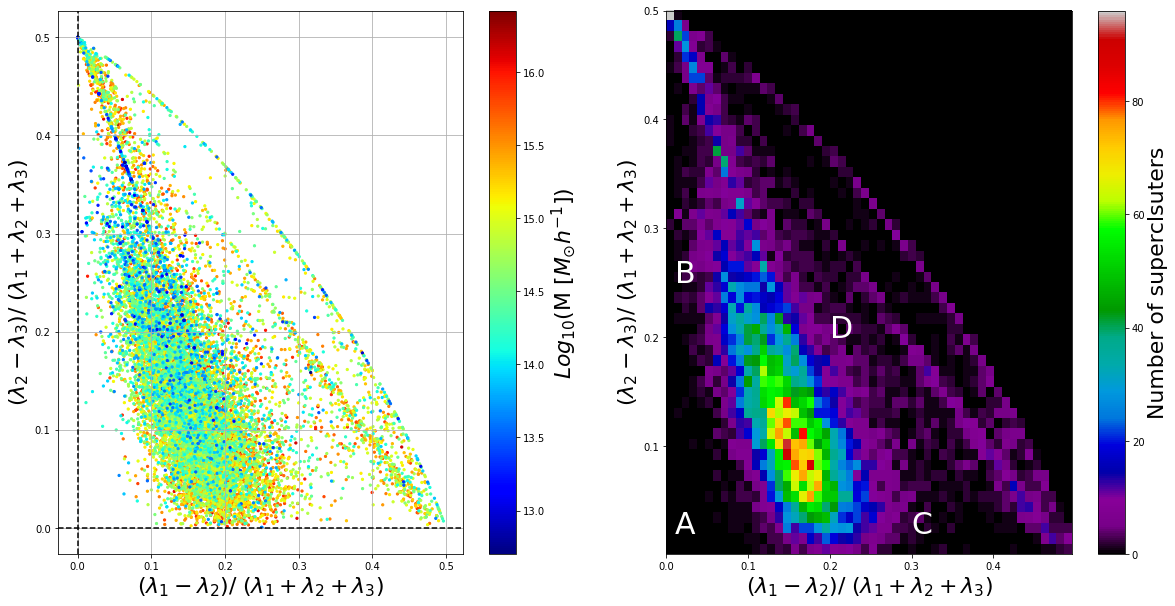
\includegraphics[width=480pt]{shapeStats_1M.png}
    \caption{On the left you can see how each supercluster is located in this space given its own moments of inertia with some notable tendency in the mass. On the right, a density distribution of the graph on the left is plotted. When all moments of inertia are equal, it is expected that the supercluster is close to region \textbf{A} in the graph corresponding to \texttt{spheres}. If the two largest semimajor axis are equal, the supercluster is in region \textbf{B} that corresponds to \texttt{prolate top} or elongated sphere. If the two smallest semimajor axis are equal, the supercluster belongs to the region \textbf{C} with the \texttt{oblate top} or oblate sphere. Region \textbf{D} belongs to those \texttt{asymmetric} superclusters whose principal moments of inertia are different from each other.}
    \label{fig:INERTIA}
\end{figure}

Keep in mind that there are superclusters that are crossing the walls of the simulation, since it is in periodic conditions, and therefore the calculation of their CM is compromised. To solve this problem each supercluster must be isolated and displaced by the axes of the simulation until an optimal displacement is found for which none of its voxels touch any wall. When the supercluster has been centered, the usual calculation of the CM is made. Once the coordinates of the center of mass have been obtained, they are displaced in the opposite direction the same distance as before and thus the position of the CM in the simulation frame is obtained.

The moments of inertia associated with the main axes are calculated and organized in such a way that $ \lambda_3 < \lambda_2 < \lambda_1 $. In order to be able to make a valid analysis on the shape, the difference between the two biggest semi-major axes and the difference between the two smallest ones is analyzed in Figure \ref{fig:INERTIA}. Taking into account that Laniakea has a flattened spheroid shape, it would be expected to be in region \textbf{C} of the right graph of Figure \ref{fig:INERTIA}. It is a relatively unpopulated region of the graph, indicating that very few superclusters share this form with laniakea. Suppose that in this distribution the oblate top superclusters correspond to all those points that lie below 0.05 on the vertical axis. The probability of finding a supercluster with these characteristics in the simulation is 7.04\%.

Laniakea, again, is found in an atypical region for a supercluster of the proposed dimensions, however, it should be noted that towards this region of the graph are more superclusters with masses similar to that registered for Laniakea by Tully et  al. \cite{tully_laniakea_2014}. This analysis was performed by Sergio Hernández in his work\cite{SHC_TESIS} obtaining similar results.




\newpage
\section{Conclusions and future work}
Modern cosmology aims to answer questions about the origin and large-scale structure of the universe. The astronomical observations already allowed us to have an idea of what the universe is like, but it was the arrival of computers and cosmological simulations that allowed us to answer more relevant questions.
A recent result in this branch was the definition of our local supercluster Laniakea made by Tully el al.(2014)\cite{tully_laniakea_2014}, who used the velocity flow of galaxies for this purpose. Already having the characteristics of Laniakea, both in form and in mass, the next question would be how common it is among the other superclusters.

We divide the space of the simulation with a grid size close to the canonical length of \texttt{10 Mpc} used in observations to find Laniakea, which corresponds to a grid of [$120 \times 120 \times 120$].Once the velocity field is obtained, it is smoothed with Gaussian kernels of different width $\sigma_{Vox}$. Then the VDC is computed for each gridpoint. In order to differentiate structures from the order of the observable superclusters i.e. structures of about 10 Mpc $h^{-1}$, we use $\sigma_{Vox} = 1$ Vox. Using larger values of $\sigma_{Vox}$ does \texttt{NOT} yield erroneous information, but information with little usefulness about formation in a much larger scale.  

The implementation of the Watershed algorithm was a complete success. It managed to segregate regions based on the divergence field. Two parameters, $R_T$ and $Q_T$, are defined to control the algorithm and the segregation it makes. $R_T$ is of high relevance since it indirectly dictates the number of \emph{origins} that there are in the map and, therefore, the number of superclusters that will be in the space of the simulation. $Q_T$, on the other hand, does not affect the analysis carried out by the algorithm in a meaningful way since it rather indirectly defines the top of watershed sweeps that must be made before proceeding to classify the voxels by distance.

With the superclusters segregated and characterized we compare their propoerties against Laniakea. We find that our supercluster is  atypical according to its mass, volume and shape. On the other hand, the density of Laniakea seems to be frequent in the supercluster population since it is in a range close to the average. The populations with which Laniakea is compared within the simulation are small, either evaluating its mass, its volume or its shape. This makes it difficult to find a supercluster in the simulation that is similar to Laniakea within the ranges defined in Figures \ref{fig:HISTVMD1} and \ref{fig:INERTIA} at the same time. The probability of finding in the simulation a supercluster similar to Laniakea in those three aspects is a little lower than 0.07\%.

Regarding future work, we strongly suggest to experiment with the initial conditions of the problem and with the definition of the grid. A proposal is to define a grid with distances less than 10 Mpc $h^{-1}$, that is, with a higher value of $N_{side}$ and therefore with greater definition. You can also try different mass cuts for the Halos, different simulations of the same cosmology used in this work or even simulations in the context of different cosmologies.\\

% Modern cosmology aims to answer questions about the origin and large-scale structure of the universe. The astronomical observations already allowed us to have an idea of what the universe is like, but it was the arrival of computers and cosmological simulations that allowed us to answer more relevant questions.
% A recent result in this branch was the definition of our local supercluster Laniakea made by Tully el al.(2014)\cite{tully_laniakea_2014}, who used the velocity flow of galaxies for this purpose. Already having the characteristics of Laniakea, both in form and in mass, the next question would be how common it is among the other superclusters.

% We divide the space of the simulation with a grid size close to the canonical length of \texttt{10 Mpc} used in observations to find Laniakea, which corresponds to a grid of [$120 \times 120 \times 120$].

% % To begin, we must talk about the methods used and how they were adjusted to the problem. dividing the space of the simulation into a grid was the frame of reference that was used to proceed with statistical analysis. This discretized the problem in a way that decreased computational calculation time and facilitated the definition of volumes in space. As previously explained, choosing the number of steps in each axis to define the grid is relevant, since although many steps mean more definition, it also means a considerable increase in computing time. Also having too many steps implies getting closer and closer to evaluating each object of the space individually, which is not the idea. A suggestion for future work would be to numerically determine this balance between the definition of the grid and the computation time required, taking into account the density of the space in order to avoid overdividing the grid. 

% % The Velocity Divergence Coefficient is a useful tool for quantifying accretion in defined regions of space. Having discretized the space with a grid, the existence of minimum units of volume, or voxels, facilitates the concept of divergence of speed. As seen in Figure \ref{fig:2D_VDC}, this scalar defines well the accretion by differentiable regions without ignoring the events of \emph{Transit Formation} mentioned in section \ref{sec:INTROVDC}. Calculating the VDC while choosing the grid as an approach to the problem was a good idea since it gave good results with a considerably good definition and  without losing much information.

% One of the decisive steps in the numerical analysis of the problem was the smoothing of the field by the Gaussian convolution method, as a filter. 
% %This smoothing was applied in the mass grid and in each one of the speed grids (one for each coordinate axis), this in  order to get consistent results and to avoid problems with the missing information of the field. 
% Depending on the width of the filter, or $\sigma_{Vox}$, diferent kinds of structures were found in the simulation space as shown in figure \ref{fig:SigmasVDCZcut}. The $\sigma_{Vox}$ value has an enormous relevance in the characterization of structures since it dictates the definition with which one wants to segregate groups. For example, to segregate structures of the approximate size of Laniakea, $\sigma_{Vox} = 1$ Vox is used, which is equivalent to structures of the order of 10 Mpc $h^{-1}$ in radius. Using superior values of $\sigma_{Vox}$ does not yield erroneous information, but information with little usefulness about formation in a much larger scale.

% The implementation of the Watershed algorithm was a total success. It managed to segregate regions based on the information that the grid $\Phi$ provided about the accretion. Two parameters, $R_T$ and $Q_T$, are defined to control the algorithm and the segregation it makes. $R_T$ is of high relevance since it indirectly dictates the number of \emph{origins} that there are in the map and, therefore, the number of superclusters that will be in the space of the simulation. $Q_T$, on the other hand, does not affect the analysis carried out by the algorithm in a meaningful way since it rather indirectly defines the top of watershed sweeps that must be made before proceeding to classify the voxels by distance. If you have enough computational power, $Q_T$ could well be zero. The reason that selecting a certain number of voxels does not significantly affect the result of segregation is that in other investigations \cite{CosmicWatershedVoidDetection} it has been determined that the classification by distance (Voronoi) is quite similar to the classification by accretion when it comes to large-scale structures. Selecting $Q_T$ as 200 Vox induces less than 0.012\% of \textit{'classification by distance'} choices. Even assuming they all are wrong, it is an small proportion compared to the size of the grid and the computational cost saved.\\

% Once the superclusters have been segregated and characterized in their great variety of forms, masses and sizes, some unknowns about the role of Laniakea in this context are being solved. Figures \ref{fig:HISTVMD1} and \ref{fig:INERTIA} summarize the result of the characterization of the superclusters and show that Laniakea is found in atypical populations according to mass, volume and shape. On the other hand, the density of Laniakea seems to be frequent in the supercluster population since it is in a range close to the average. The populations with which Laniakea is compared within the simulation are small, either evaluating its mass, its volume or its shape. This makes it difficult to find a supercluster in the simulation that is similar to Laniakea within the ranges defined in Figures \ref{fig:HISTVMD1} and \ref{fig:INERTIA} at the same time. The probability of finding in the simulation a supercluster similar to Laniakea in those three aspects is a little lower than 0.07\%.
\newpage
%\section{References\label{sec:references}}

\bibliographystyle{unsrt}
\bibliography{References}

\newpage
.
\vspace{10cm}


\begin{tabular}{@{}p{.5in}p{4in}@{}}
& \hrulefill \\
& Jaime E. Forero.Romero, Ph.D. \\
& Universidad de los Andes, Departamento de Física\\
& \\
& \\
& \\
& \hrulefill \\
& David Leonardo Paipa León \\
& Universidad de los Andes, Departamento de Física\\

\end{tabular}

\end{document}













%===================================================================
% Your introduction goes here! Some examples of commonly used commands and features are listed below, to help you get started.

% If you have a question, please use the support box in the bottom right of the screen to get in touch. 

% \section{Some \LaTeX{} Examples}
% \label{sec:examples}

% \subsection{Sections}

% Use section and subsection commands to organize your document. \LaTeX{} handles all the formatting and numbering automatically. Use ref and label commands for cross-references.

% \subsection{Comments}

% Comments can be added to the margins of the document using the \todo{Here's a comment in the margin!} todo command, as shown in the example on the right. You can also add inline comments too:

% \todo[inline, color=green!40]{This is an inline comment.}

% \subsection{Tables and Figures}

% Use the table and tabular commands for basic tables --- see Table~\ref{tab:widgets}, for example. You can upload a figure (JPEG, PNG or PDF) using the files menu. To include it in your document, use the includegraphics command as in the code for Figure~\ref{fig:frog} below.

% % Commands to include a figure:
% \begin{figure}
% \centering
% \includegraphics[width=0.5\textwidth]{frog.jpg}
% \caption{\label{fig:frog}This is a figure caption.}
% \end{figure}

% \begin{table}
% \centering
% \begin{tabular}{l|r}
% Item & Quantity \\\hline
% Widgets & 42 \\
% Gadgets & 13
% \end{tabular}
% \caption{\label{tab:widgets}An example table.}
% \end{table}

% \subsection{Mathematics}

% \LaTeX{} is great at typesetting mathematics. Let $X_1, X_2, \ldots, X_n$ be a sequence of independent and identically distributed random variables with $\text{E}[X_i] = \mu$ and $\text{Var}[X_i] = \sigma^2 < \infty$, and let
% $$S_n = \frac{X_1 + X_2 + \cdots + X_n}{n}
%       = \frac{1}{n}\sum_{i}^{n} X_i$$
% denote their mean. Then as $n$ approaches infinity, the random variables $\sqrt{n}(S_n - \mu)$ converge in distribution to a normal $\mathcal{N}(0, \sigma^2)$.

% \subsection{Lists}

% You can make lists with automatic numbering \dots

% \begin{enumerate}
% \item Like this,
% \item and like this.
% \end{enumerate}
% \dots or bullet points \dots
% \begin{itemize}
% \item Like this,
% \item and like this.
% \end{itemize}

% We hope you find write\LaTeX\ useful, and please let us know if you have any feedback using the help menu above.
